\documentclass[11pt,a4paper]{article}

% Derleyici: XeLaTeX (Overleaf: Menu -> Compiler -> XeLaTeX)
\usepackage{fontspec}
\usepackage{polyglossia}
\setmainlanguage{turkish}

\usepackage[a4paper,margin=2.5cm]{geometry}
\usepackage{graphicx}
\usepackage{booktabs}
\usepackage{tabularx}
\usepackage{longtable}
\usepackage{array}
\usepackage{float}
\usepackage{listings}
\usepackage{xcolor}
\usepackage{enumitem}
\usepackage{caption}
\usepackage{titlesec}
\usepackage{fancyhdr}
\usepackage{hyperref}
\usepackage{setspace}

\hypersetup{colorlinks=true, linkcolor=blue!50!black, urlcolor=blue!50!black}
\setlength{\parindent}{0pt}
\setlength{\parskip}{0.45em}
\onehalfspacing
\pagestyle{fancy}
\fancyhf{}
\fancyhead[L]{\small BIL372 --- Mini-Dealership Son Rapor}
\fancyfoot[C]{\thepage}

\newcommand{\kod}[1]{\texttt{\detokenize{#1}}}
\newcommand{\sekil}[1]{Şekil~\ref{#1}}
\newcommand{\tablo}[1]{Tablo~\ref{#1}}

\lstset{
  basicstyle=\ttfamily\small,
  breaklines=true,
  frame=single,
  columns=fullflexible,
  keepspaces=true,
  showstringspaces=false,
  backgroundcolor=\color{gray!5},
  rulecolor=\color{gray!40},
}

\title{Mini-Dealership\\[0.3em]
\large Çok Şubeli Otomobil Bayisi için WhatsApp Randevu Asistanı ve Yönetim Paneli\\[0.6em]
\normalsize PROJE SON RAPORU}
\author{Hüseyin Yiğit USTA --- 231101041\\ Şevda Yağmur ASAL --- 221104100}
\date{27 Kasım 2026}

\begin{document}

\begin{titlepage}
\centering
\vspace*{2.5cm}
{\Large TOBB EKONOMİ VE TEKNOLOJİ ÜNİVERSİTESİ\par}
{\large BİLGİSAYAR MÜHENDİSLİĞİ BÖLÜMÜ\par}
{\large BIL372 Veritabanı Sistemleri\par}
\vspace{2cm}
{\Huge\bfseries Mini-Dealership\par}
\vspace{0.6cm}
{\Large Çok Şubeli Otomobil Bayisi için\\ WhatsApp Randevu Asistanı ve Yönetim Paneli\par}
\vspace{1.2cm}
{\Large\bfseries PROJE SON RAPORU\par}
\vfill
\begin{tabular}{ll}
Hüseyin Yiğit USTA & 231101041\\
Şevda Yağmur ASAL & 221104100\\
\end{tabular}\\[1cm]
{\large 27 Kasım 2026\par}
\end{titlepage}

\tableofcontents
\newpage

% =====================================================================
\section{Gerçek Dünya Probleminin Tanımı}

Çok şubeli bir otomobil bayisinde randevu yönetimi telefon, elle yazılan WhatsApp
mesajları ve şube bazında tutulan Excel dosyalarıyla yürütülmektedir. Bu düzenin
ölçülebilir sonuçları şunlardır:

\begin{itemize}[leftmargin=1.2em]
  \item Mesai dışında gelen mesajlar cevapsız kalır; müşteri başka bir kanala yönelir.
  \item Şubeler birbirinin müsaitliğini görmediği için aynı çalışana veya araca
        çakışan randevu verilebilir.
  \item Yetkisi olmayan bir çalışana test sürüşü yazılabilir; stokta olmayan ya da
        müşterinin kendi aracı olmayan bir araç için servis randevusu açılabilir.
  \item Veri dağınık olduğu için ``hangi model çok test ediliyor ama satılmıyor?``,
        ``hangi şube serviste gecikiyor?`` gibi sorular cevaplanamaz.
  \item Randevu, mesaj ve stok hareketi kayıtları yüz binlere ulaştığından,
        tutarlılığı uygulama koduna bırakmak sürdürülebilir değildir.
\end{itemize}

Projenin amacı; müşterinin tek bir WhatsApp hattından randevu alabildiği, bayinin
aynı veriyi bir web panelinden yönettiği ve tüm iş kurallarının \textbf{veritabanında}
garanti edildiği bir sistemi uçtan uca kurmaktır.

\subsection{Sistemin kapsamı}

Sistem dört parçadan oluşur:

\begin{table}[H]
\centering
\small
\begin{tabularx}{\textwidth}{@{}l l X@{}}
\toprule
Parça & Teknoloji & Görev\\
\midrule
WhatsApp köprüsü & Node.js + Baileys & Mesajı backend'e iletir, cevabı gönderir; DB'ye dokunmaz\\
Backend & Java 17, JDBC (ORM yok) & Bot API, panel API, iş kuralları, transaction, LLM araç döngüsü\\
Panel & HTML/CSS/JS (düz) & Personel arayüzü; backend tarafından aynı kökenden sunulur\\
Veritabanı & PostgreSQL 17 & 20 tablo, 7 view, roller/RLS, trigger ve EXCLUDE kısıtları\\
\bottomrule
\end{tabularx}
\caption{Sistem bileşenleri}
\label{tab:bilesenler}
\end{table}

Dil modeli yalnızca \textbf{doğal dil anlama ve yönlendirme} için kullanılır.
Randevu kuralları (mesai, tür saat penceresi, yetkinlik, çakışma, sahiplik) modele
bırakılmaz; \kod{CHECK}, \kod{EXCLUDE}, trigger ve rol/RLS ile veritabanında uygulanır.

% =====================================================================
\section{Gereksinim Analizi}

\subsection{Aktörler}

\begin{table}[H]
\centering
\small
\begin{tabularx}{\textwidth}{@{}l X l@{}}
\toprule
Aktör & Temsil & Yetki\\
\midrule
Müşteri & WhatsApp telefonu & Stok, kendi randevuları, iptal, randevu alma\\
Satış personeli & Panel oturumu (\kod{personel}) & Randevu, araç, müşteri, rapor okuma\\
Servis personeli & Panel oturumu (\kod{personel}) & Servis kaydı, durum ve masraf işlemleri\\
Rapor kullanıcısı & Panel oturumu (\kod{rapor}) & Yalnız maskeli view'lar ve Excel\\
Bot & \kod{bot} DB rolü + \kod{X-Bot-Token} & Yalnız konuştuğu müşterinin satırları (RLS)\\
Yönetici & \kod{admin} (şema sahibi) & Şema ve rol yönetimi\\
\bottomrule
\end{tabularx}
\caption{Aktörler ve yetkiler}
\label{tab:aktorler}
\end{table}

\subsection{İşlevsel gereksinimler}

\begin{longtable}{@{}p{0.7cm} p{6.2cm} p{7.4cm}@{}}
\toprule
\# & Gereksinim & Gerçekleme\\
\midrule
\endhead
G1 & Müşteri telefonla tanınır, yeni müşteri açılır & \kod{musteri.telefon UNIQUE}; bot \kod{POST /bot/musteri}\\
G2 & Şehir/şube ve tür bazında boş saat önerilir & \kod{v_dolu_slot}, \kod{GET /bot/slot}\\
G3 & Randevu oluşturma; çakışma, mesai, yetkinlik denetimi & \kod{220_trg_randevu_dogrula}, EXCLUDE\\
G4 & Müşteri kendi randevularını görür/iptal eder & RLS + \kod{GET /bot/randevu}, \kod{POST .../iptal}\\
G5 & Stok ve yoldaki araçlar bildirilir & \kod{GET /bot/arac}, \kod{v_arac_garanti_durumu}\\
G6 & Panelden randevu eklenir, durum değiştirilir & \kod{POST /panel/randevu}, \kod{POST .../durum}\\
G7 & Araç, müşteri, servis kaydı izlenir & \kod{GET /panel/arac}, \kod{/musteri}, \kod{/servis}\\
G8 & Servis durum geçmişi ve masraf/ödeme kaynağı & \kod{servis_durum_gecmisi}, \kod{servis_islem}, \kod{210} trigger\\
G9 & Garanti saklanmaz, hesaplanır & \kod{v_arac_garanti_durumu} (1 yıl / 15.000 km)\\
G10 & Rapor özeti ve tek yönlü Excel & \kod{GET /panel/rapor/ozet}, \kod{.../randevu.xlsx}\\
G11 & Bot konuşmaları panelde görünür & \kod{GET /panel/musteri/{id}/mesaj}\\
G12 & WhatsApp'tan doğal dilde randevu & \kod{POST /bot/mesaj} + LLM araç döngüsü\\
\bottomrule
\caption{İşlevsel gereksinimler}
\label{tab:gereksinimler}
\end{longtable}

\subsection{İşlevsel olmayan gereksinimler}

\begin{table}[H]
\centering
\small
\begin{tabularx}{\textwidth}{@{}l X@{}}
\toprule
\# & Gereksinim ve karşılanma\\
\midrule
N1 & Veri tutarlılığı uygulama hatasından bağımsız: kısıt + trigger + EXCLUDE\\
N2 & PII minimizasyonu: TC/kimlik yok; bot yalnız kendi müşterisi; rapor maskeli view\\
N3 & Yetki ayrımı: \kod{admin/personel/bot/rapor}; hiçbir rolde DELETE yok\\
N4 & Eşzamanlılık: EXCLUDE + transaction; müşteri upsert; oturum kilidi\\
N5 & Ölçek: 660.433 satır sentetik veri; 13 indeks; ölçülen planlar\\
N6 & Güvenlik: parametreli SQL, token, bcrypt, CSP, path traversal savunması\\
N7 & Tekrarlanabilirlik: numaralı \kod{db/*.sql}, \kod{veri/uret.py}, test betikleri\\
N8 & Bakım: ORM yok; SQL dosyaları ve handler'lar ayrı sorumluluklar\\
\bottomrule
\end{tabularx}
\caption{İşlevsel olmayan gereksinimler}
\label{tab:nfr}
\end{table}

\subsection{Varsayımlar ve kapsam dışı}

\begin{itemize}[leftmargin=1.2em]
  \item Bayi tek markalıdır; markanın bütün araçları bayi ağından satılır, servise
        gelen her araç sistemde kayıtlıdır.
  \item Mesai ve randevu türü saat pencereleri tüm şubelerde ortaktır.
  \item Ödeme şubede yüz yüze alınır; sistem yalnızca masraf/ödeme kaynağını kaydeder.
  \item Kapsam dışı: panelden satış transaction'ı (\kod{POST /panel/satis}) ve servis
        kaydı açma uçları. Bunlar tasarımda yer alır; demo kapsamında randevu ve
        servis takibi üzerinden gösterilir.
\end{itemize}

% =====================================================================
\section{Kavramsal Tasarım (EER)}

Kavramsal model ara raporda ayrıntılı verilmiştir. Son uygulamada değişmeyen ana
kararlar:

\begin{itemize}[leftmargin=1.2em]
  \item \textbf{Kalıtım:} Randevu alt sınıfları tek tabloda, ayırt edici
        \kod{tur_kodu} ile tutulur. Böylece çalışan/araç/müşteri çakışması bütün
        randevu türleri için tek EXCLUDE kısıtıyla engellenir. Alt sınıfa özgü
        \kod{arac_vin}/\kod{versiyon_id} zorunluluğu CHECK ile türe bağlanır.
  \item \textbf{Çoka-çok:} \kod{calisan_yetkinlik} (çalışan $\times$ yetkinlik),
        veriliş/bitiş tarihiyle.
  \item \textbf{Türetilmiş nitelikler:} Garanti durumu, son bakım, doluluk ve kalan
        gün saklanmaz; view'larda hesaplanır.
  \item \textbf{Zayıf varlık:} \kod{servis_durum_gecmisi} servis kaydına bağlıdır;
        kimliği \kod{(servis_kaydi_id, zaman)} benzersizliğiyle desteklenir.
  \item \textbf{Silmeli tasarım yok:} İptal, durum değişikliğidir; çalışan ayrılırsa
        \kod{aktif_mi=false} olur. Hiçbir uygulama rolünde DELETE yetkisi yoktur.
\end{itemize}

\begin{figure}[H]
\centering
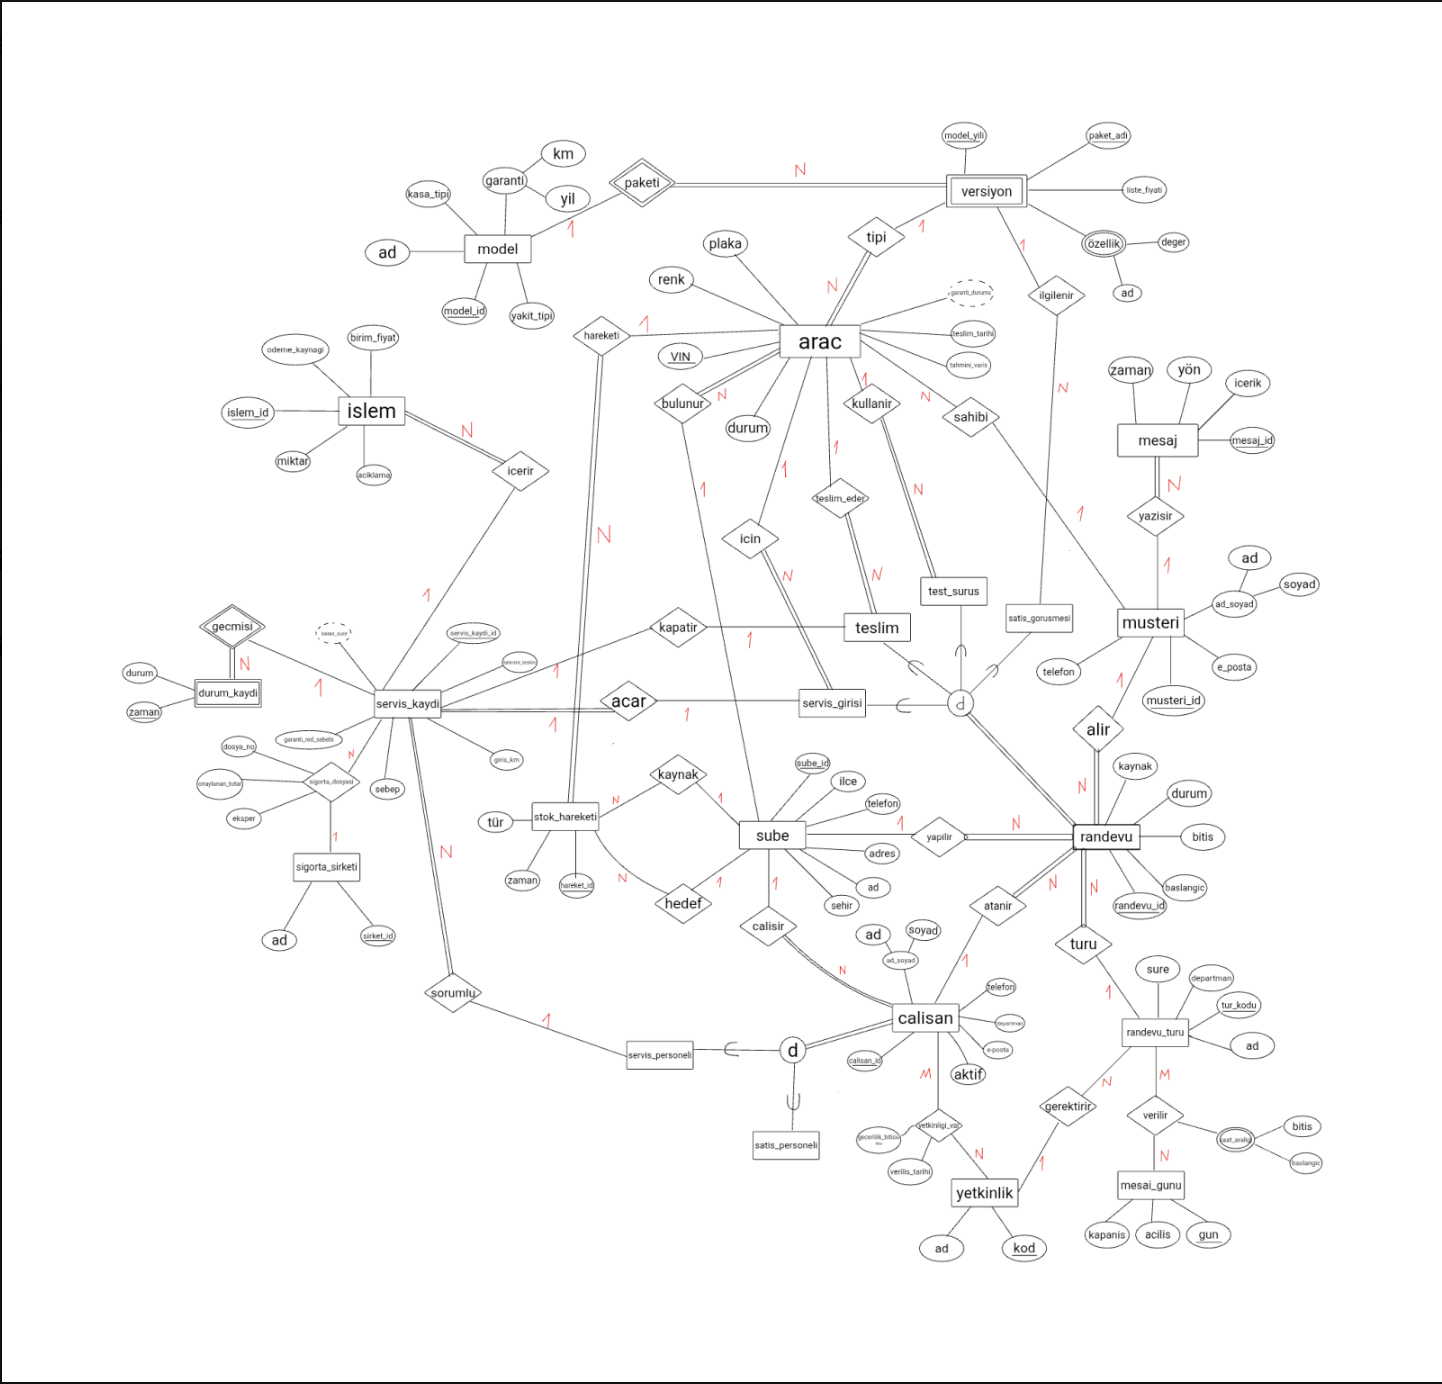
\includegraphics[width=0.82\textwidth]{figures/eer.png}
\caption{EER diyagramı (ara rapor, Şekil 1)}
\label{fig:eer}
\end{figure}

% =====================================================================
\section{Mantıksal Tasarım ve Şema}

\subsection{Tablolar}

Şema 20 tablodan oluşur. Özet:

\footnotesize
\begin{longtable}{@{}>{\raggedright\arraybackslash}p{2.9cm} >{\raggedright\arraybackslash}p{3.7cm} >{\raggedright\arraybackslash}p{7.6cm}@{}}
\toprule
Tablo & Birincil anahtar & Önemli kısıt\\
\midrule
\endhead
\kod{sube} & \kod{sube_id} & \kod{UNIQUE (sehir, ad)}\\
\kod{mesai} & \kod{gun} & \kod{acilis < kapanis}\\
\kod{yetkinlik} & \kod{yetkinlik_id} & \kod{UNIQUE kod}\\
\kod{calisan} & \kod{calisan_id} & \kod{UNIQUE eposta}, \kod{UNIQUE kullanici_adi}; departman\\
\kod{calisan_yetkinlik} & \kod{(calisan_id, yetkinlik_id)} & Veriliş/bitiş tarihi\\
\kod{model} & \kod{model_id} & \kod{UNIQUE ad}; garanti yıl/km\\
\kod{versiyon} & \kod{versiyon_id} & \kod{UNIQUE (model_id, paket_adi, model_yili)}\\
\kod{versiyon_ozellik} & \kod{(versiyon_id, ozellik_adi)} & CASCADE\\
\kod{musteri} & \kod{musteri_id} & \kod{UNIQUE telefon}; ad/soyad NULL olabilir\\
\kod{mesaj} & \kod{mesaj_id} & yön; \kod{kaynak_id} idempotency\\
\kod{arac} & \kod{vin} & \kod{UNIQUE plaka}; durum $\in$ \{YOLDA, STOKTA, SATILDI\}\\
\kod{stok_hareketi} & \kod{hareket_id} & tür $\in$ \{SIPARIS, GELIS, TRANSFER, SATIS\}\\
\kod{randevu_turu} & \kod{tur_kodu} & Süre, departman, yetkinlik\\
\kod{tur_saat} & \kod{(tur_kodu, gun, baslangic)} & Aralık mesai içinde\\
\kod{randevu} & \kod{randevu_id} & EXCLUDE: çalışan/araç/müşteri çakışması\\
\kod{servis_kaydi} & \kod{servis_kaydi_id} & Açılış/teslim randevusu UNIQUE; sebep\\
\kod{servis_durum_gecmisi} & \kod{gecmis_id} & \kod{UNIQUE (servis_kaydi_id, zaman)}\\
\kod{servis_islem} & \kod{islem_id} & Ödeme kaynağı sebebe göre\\
\kod{sigorta_sirketi} & \kod{sirket_id} & \kod{UNIQUE ad}\\
\kod{servis_sigorta} & \kod{servis_kaydi_id} & \kod{UNIQUE (sirket_id, dosya_no)}\\
\bottomrule
\caption{Tablolar, anahtarlar ve kısıtlar}
\label{tab:tablolar}
\end{longtable}
\normalsize

\begin{figure}[H]
\centering
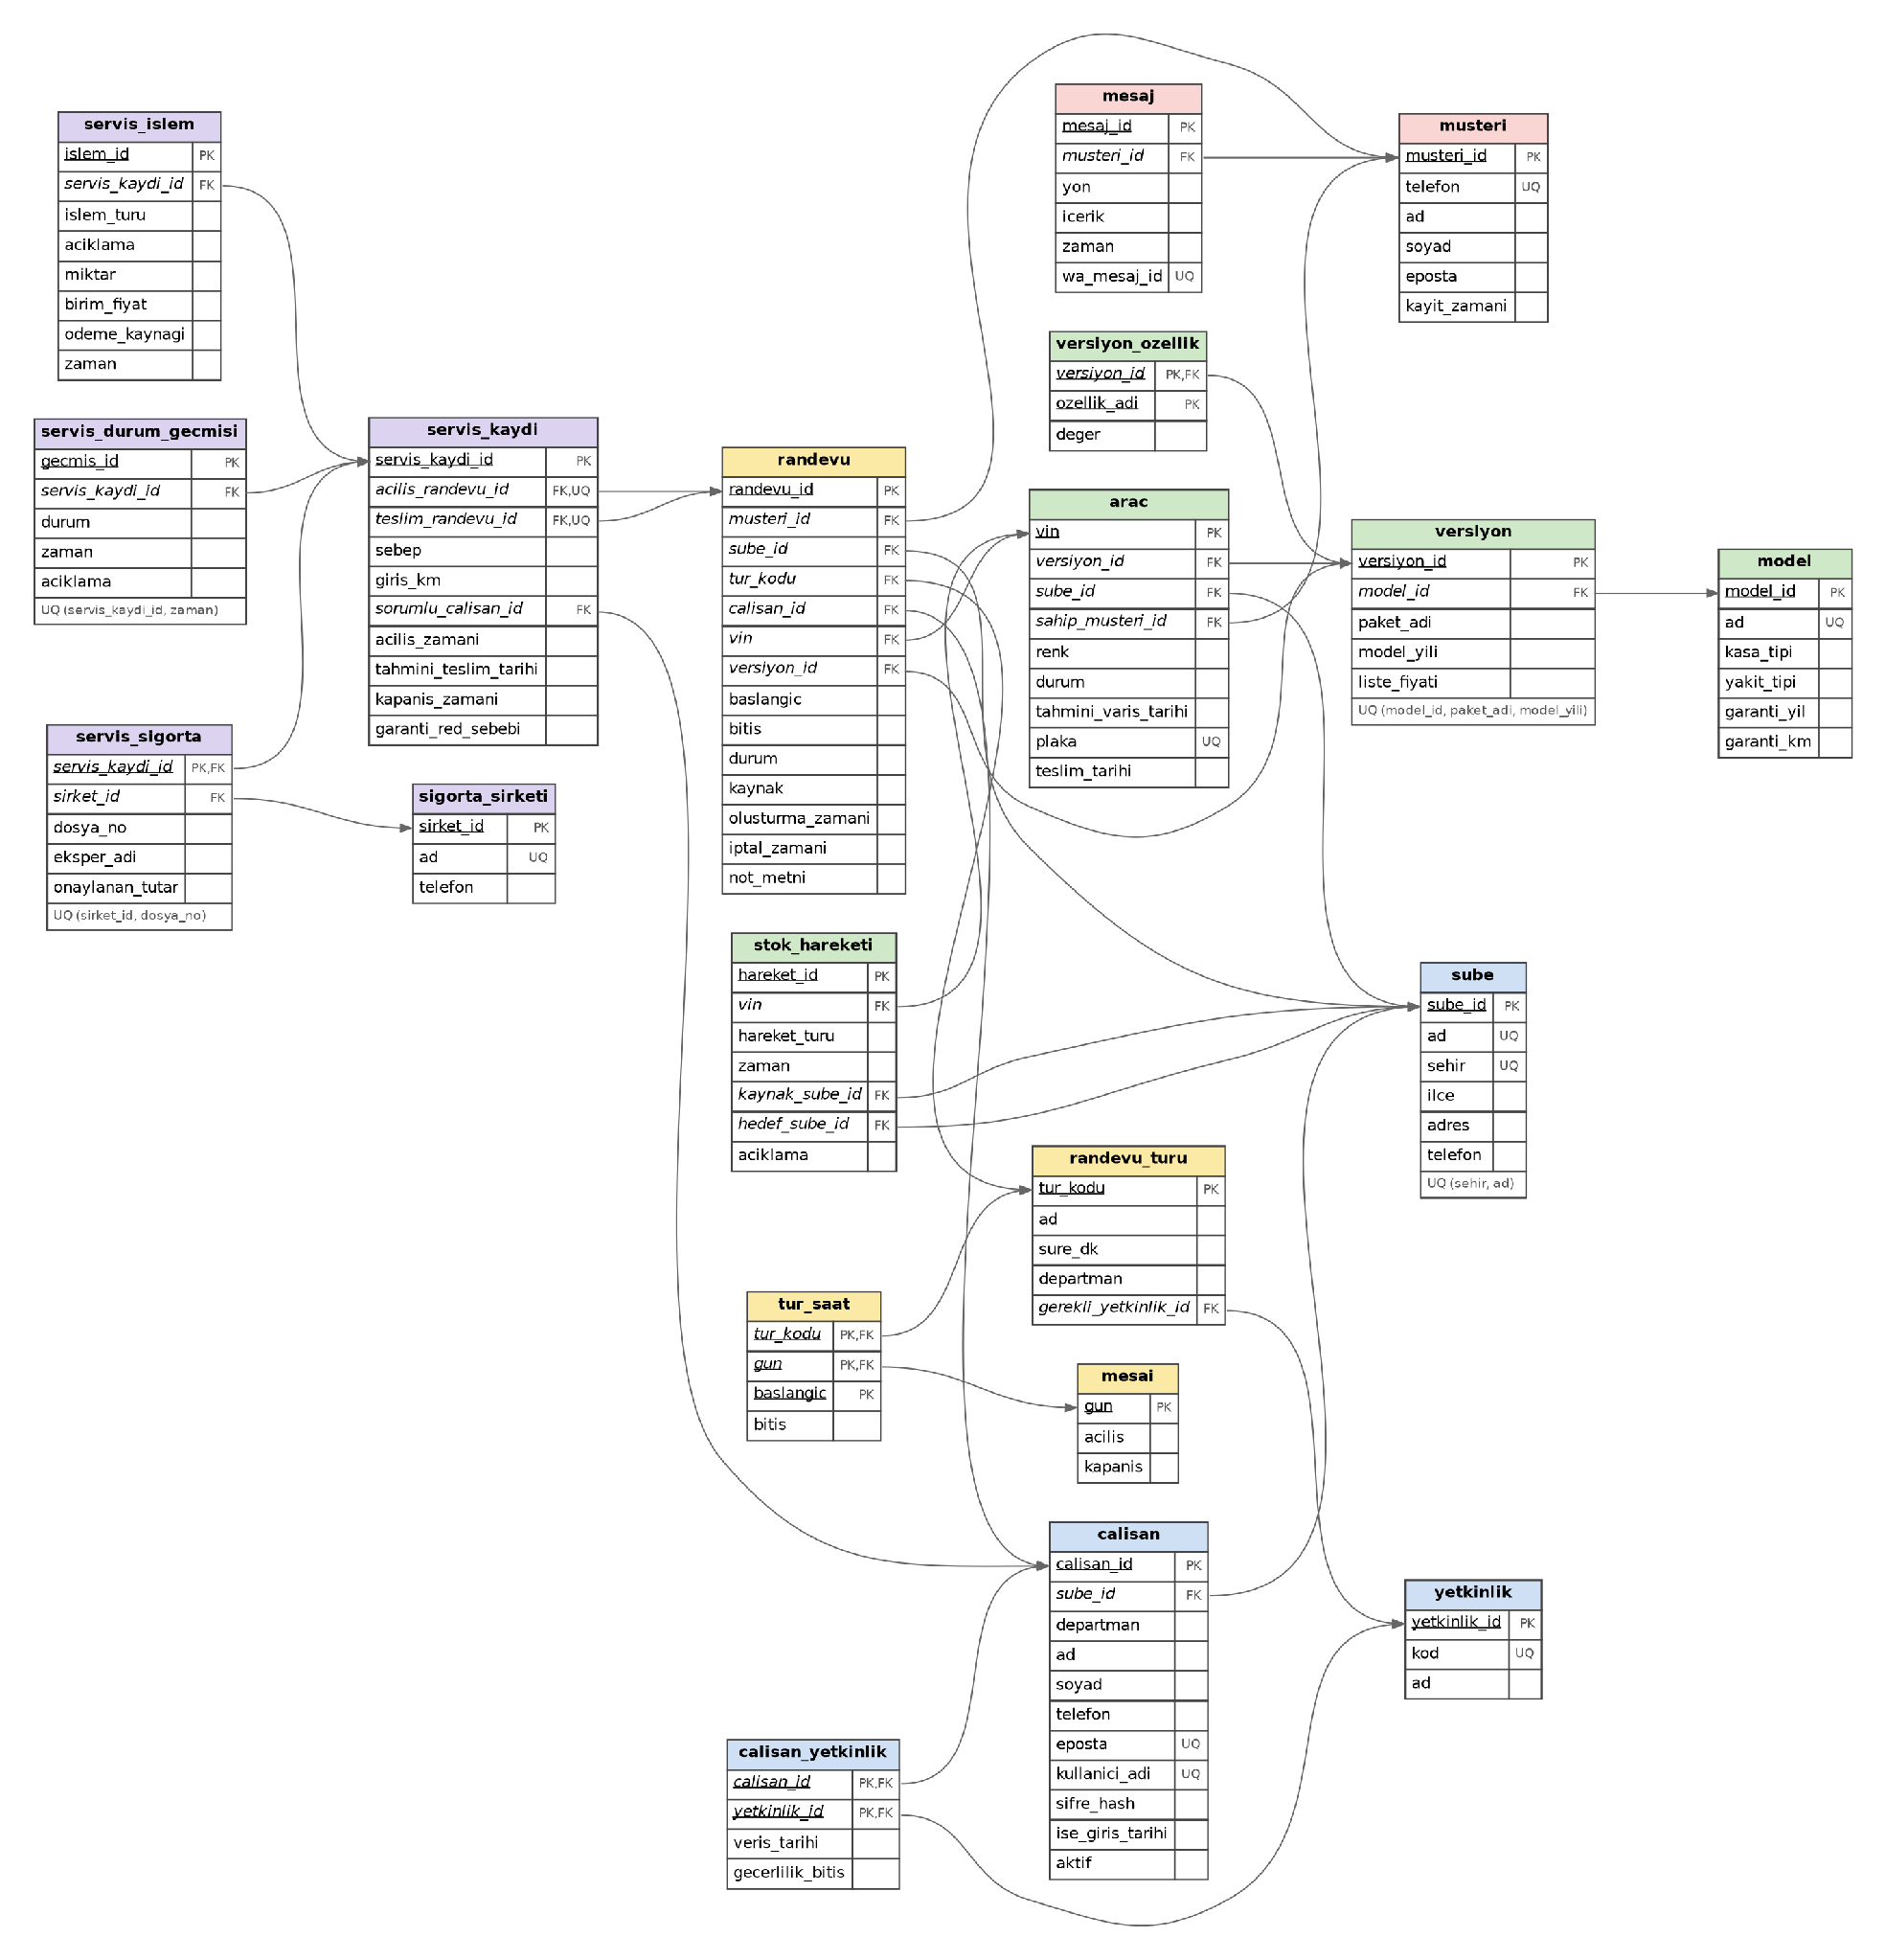
\includegraphics[width=0.86\textwidth]{figures/sema.png}
\caption{İlişkisel şema}
\label{fig:sema}
\end{figure}

\subsection{Bütünlük kuralları}

\begin{itemize}[leftmargin=1.2em]
  \item \textbf{EXCLUDE (GiST):} Aynı çalışan, araç veya müşteri için örtüşen
        \kod{tsrange} aralığı yasaktır. \kod{btree_gist} uzantısı eşitlik + aralık
        için kullanılır.
  \item \textbf{\kod{220_trg_randevu_dogrula}:} Mesai/tür saat penceresi, çalışanın
        şubesi, departmanı, yetkinliği ve aktifliği; araç türüne göre durum.
  \item \textbf{\kod{460_trg_randevu_sahiplik}:} Araç müşterinin kendi aracı olmalı;
        servisten teslimde açık ve TESLİME HAZIR servis kaydı bulunmalı.
        \kod{CONSTRAINT TRIGGER DEFERRABLE} olarak tanımlıdır: sentetik veri tek
        transaction'da önce randevuları yazabilsin, kural commit'te doğrulansın.
        Yalnız durum güncelleyen UPDATE'ler yeniden doğrulanmaz.
  \item \textbf{\kod{210_trg_servis_garanti}:} Garantisi düşmüş araca ``garanti''
        ödemesi girilemez; ödeme kaynağı sebebe göre sınırlıdır.
  \item \textbf{CHECK'ler:} Para kolonları \kod{bigint} tam TL; durum kolonları
        \kod{varchar + CHECK}; araç durumuna göre plaka/sahip zorunluluğu.
\end{itemize}

\subsection{View'lar}

\begin{table}[H]
\centering
\small
\begin{tabularx}{\textwidth}{@{}l X@{}}
\toprule
View & Amaç\\
\midrule
\kod{v_musteri_son_randevu} & Müşterinin iptaller hariç son randevusu\\
\kod{v_servis_durumu} & Servis kaydının son durumu, kalan gün, gecikme, toplam masraf\\
\kod{v_arac_garanti_durumu} & Satıştan itibaren garanti ve son bakım (hesaplanır)\\
\kod{v_rapor_randevu} & \kod{rapor} rolü için maskeli randevu satırları\\
\kod{v_rapor_musteri} & \kod{rapor} rolü için maskeli müşteri satırları\\
\kod{v_dolu_slot} & Bot için PII'siz dolu saatler\\
\kod{v_musteri_servis_durumu} & Bot için müşteriye özel, masrafsız servis durumu\\
\bottomrule
\end{tabularx}
\caption{View'lar}
\label{tab:viewlar}
\end{table}

\subsection{Normalizasyon}

Şema BCNF'ye kadar normalleştirilmiştir. Öne çıkan ayrıştırmalar:

\begin{itemize}[leftmargin=1.2em]
  \item \kod{model} $\leftrightarrow$ \kod{versiyon} $\leftrightarrow$
        \kod{versiyon_ozellik}: Donanım paketi ve özellikler tekrar etmez.
  \item \kod{randevu_turu} $\leftrightarrow$ \kod{tur_saat}: Türün süresi ve gün
        bazlı saat pencereleri ayrı tutulur.
  \item \kod{servis_kaydi} $\leftrightarrow$ \kod{servis_durum_gecmisi}
        $\leftrightarrow$ \kod{servis_islem}: Olay geçmişi ve masraf kalemleri ayrı;
        geçmiş yalnızca eklenir.
  \item \kod{sigorta_sirketi} $\leftrightarrow$ \kod{servis_sigorta}: Şirket bilgisi
        tekrar etmez.
  \item Türetilmiş alanlar (garanti, son bakım, doluluk) saklanmaz; view'da hesaplanır.
\end{itemize}

% =====================================================================
\section{Tasarımın Uyarlanması}

\subsection{Mimari}

{\small
\begin{verbatim}
WhatsApp --> kopru (Node.js + Baileys) --HTTP--> backend (Java 17, JDK HttpServer)
                                                   |  JDBC (HikariCP, ORM yok)
                                                   v
                                             PostgreSQL 17
                                                   ^
Panel (tarayici) --HTTP (Bearer oturum)------------+
\end{verbatim}
}

\begin{itemize}[leftmargin=1.2em]
  \item \textbf{Köprü DB'ye dokunmaz.} Mesajı \kod{POST /bot/mesaj}'a bırakır;
        backend LLM'i ve araçları çalıştırır, cevabı döner.
  \item \textbf{Backend} bot ve panel uçlarını aynı süreçte sunar. Panel için ayrı,
        \kod{NOINHERIT} bir login rolü kullanılır; her istek \kod{SET LOCAL ROLE}
        ile yetkilendirilir.
  \item \textbf{Panel} aynı kökenden sunulur: CORS yok, oturum anahtarı başka
        kökene gitmez.
\end{itemize}

\subsection{Yazılım, donanım ve VTYS ortamı}

\begin{table}[H]
\centering
\small
\begin{tabularx}{\textwidth}{@{}l X@{}}
\toprule
Bileşen & Sürüm / seçim\\
\midrule
İşletim sistemi (geliştirme) & macOS (Apple Silicon)\\
Java & OpenJDK 17, Maven Wrapper\\
PostgreSQL & 17 (Docker \kod{postgres:17-alpine})\\
Node.js & 22 (köprü)\\
Baileys & 7.0.0-rc13\\
HTTP & JDK \kod{com.sun.net.httpserver} (ek çatı yok)\\
JDBC & PostgreSQL JDBC + HikariCP\\
JSON & Jackson\\
Şifre & jBCrypt (cost 10)\\
Excel & fastexcel (tek yönlü üretim)\\
LLM & Mistral (demo: \kod{deepseek-v4-1-flash-1017}) / Gemini (yedek)\\
\bottomrule
\end{tabularx}
\caption{Uygulama ortamı}
\label{tab:ortam}
\end{table}

\subsection{Tabloların oluşturulması}

DDL, \kod{db/} altında sayı önekli dosyalarla sırayla uygulanır:

\begin{table}[H]
\centering
\small
\begin{tabularx}{\textwidth}{@{}l X@{}}
\toprule
Aralık & İçerik\\
\midrule
\kod{010}--\kod{100} & Şema, uzantılar, ortak tipler, 20 tablo\\
\kod{150}--\kod{210} & Randevu türleri, servis/garanti trigger'ları\\
\kod{220} & Randevu doğrulama trigger'ı\\
\kod{300}--\kod{350} & View'lar ve maskeleme fonksiyonları\\
\kod{400}--\kod{430} & Roller, RLS, GRANT/REVOKE, bot kimliği\\
\kod{440} & Müşteri ad/soyad NULL gevşetmesi + bot UPDATE\\
\kod{450} & Mesaj idempotency (\kod{kaynak_id})\\
\kod{460} & Randevu--araç sahipliği ve servis hazırlığı\\
\kod{500} & 13 indeks\\
\bottomrule
\end{tabularx}
\caption{DDL dosyaları}
\label{tab:ddl}
\end{table}

Tablolar \kod{GENERATED ALWAYS AS IDENTITY} birincil anahtar kullanır; silme yerine
durum/aktiflik tercih edilir.

\subsection{View'lar ve maskeleme}

\begin{itemize}[leftmargin=1.2em]
  \item \kod{v_rapor_randevu}, \kod{v_rapor_musteri}: \kod{fn_maskele_ad} ve
        \kod{fn_maskele_telefon} ile PII maskelenir; \kod{rapor} rolü ham tabloları
        okuyamaz.
  \item \kod{v_dolu_slot}: yalnızca \kod{arac_vin}, \kod{baslangic}, \kod{bitis};
        müşteri/çalışan bilgisi yok.
  \item \kod{v_musteri_servis_durumu}: \kod{fn_aktif_musteri_id()} ile yalnız
        konuşulan müşterinin satırları; masraf ve çalışan bilgisi yok (fail-closed).
\end{itemize}

\subsection{Veri yükleme}

\kod{veri/uret.py} ile üretilen CSV'ler \kod{veri/uretilen/} altına yazılır;
\kod{scripts/veri-yukle.sh} tek transaction'da \verb|\copy| ile yükler.

\begin{table}[H]
\centering
\small
\begin{tabular}{@{}l r@{}}
\toprule
Tablo & Satır\\
\midrule
\kod{mesaj} & 216.782\\
\kod{servis_islem} & 139.005\\
\kod{servis_durum_gecmisi} & 134.549\\
\kod{randevu} & 77.961\\
\kod{servis_kaydi} & 32.989\\
\kod{musteri} & 25.339\\
\kod{stok_hareketi} & 23.804\\
\kod{arac} & 8.064\\
Diğer 12 tablo & 2.940\\
\midrule
\textbf{Toplam} & \textbf{660.433}\\
\bottomrule
\end{tabular}
\caption{Sentetik veri hacmi}
\label{tab:veri}
\end{table}

Ana işlem tablolarındaki satır sayısı \textbf{453.096}'dır (koşul: $\ge$ 250.000).
Kimlik sayaçları yükleme öncesi sıfırlanır; yükleme tek transaction olduğu için
kurala uymayan tek satır tüm işlemi geri alır. \kod{460} trigger'ı DEFERRABLE olduğu
için randevular servis kayıtlarından önce yazılabilir; kural commit'te doğrulanır.

\subsection{İndeksler}

\kod{db/500_indeksler.sql} 13 indeks tanımlar:

\begin{itemize}[leftmargin=1.2em]
  \item \kod{randevu}: şube+tarih, çalışan+tarih, müşteri, araç (kısmi), GiST EXCLUDE.
  \item \kod{mesaj}: müşteri+zaman, kaynak id (kısmi UNIQUE).
  \item \kod{servis_kaydi} / \kod{servis_islem} / \kod{servis_durum_gecmisi}:
        kayıt ve zaman.
  \item \kod{stok_hareketi}: araç+zaman.
  \item \kod{musteri}: telefon (UNIQUE zaten), kayıt zamanı.
\end{itemize}

Ölçüm: \kod{docs/analiz/indeks-analizi.md}, \kod{docs/analiz/sorgular.sql}.

\subsection{Sorgu tasarımları ve maliyet analizi}

Yedi analitik sorgu (en az 3 tablo JOIN, alt sorgu, GROUP BY/HAVING veya pencere
fonksiyonu) ve bir view ölçümü \kod{EXPLAIN (ANALYZE, BUFFERS)} ile ölçüldü.

\begin{table}[H]
\centering
\small
\begin{tabularx}{\textwidth}{@{}c X r r r@{}}
\toprule
Sorgu & Amaç & İndekssiz & İndeksli & Kazanç\\
\midrule
1 & Test sürüşü $\rightarrow$ satış dönüşümü & 14,92 ms & 8,52 ms & 1,75$\times$\\
2 & Şube/departman aylık performans & 3,04 ms & 0,35 ms & 8,7$\times$\\
3 & 216k mesajda müşteri geçmişi & 4,82 ms & 0,50 ms & 9,6$\times$\\
4 & Şube/sebep masraf kırılımı & 7,94 ms & 2,91 ms & 2,7$\times$\\
5 & Servis teslim gecikmesi & --- & 22,44 ms & Hash Join\\
6 & Garanti karşılama oranı & 111,40 ms & 108,81 ms & CPU-bound (LAG)\\
7 & Erken garanti bozulması & --- & 97,18 ms & Pencere fonksiyonu\\
8 & Müşteri servis durumu view'ı & 416,88 ms & 0,58 ms & 722$\times$\\
\bottomrule
\end{tabularx}
\caption{Sorgu maliyeti karşılaştırması}
\label{tab:sorgular}
\end{table}

Sorgu 8'in 722$\times$ kazancı, \kod{v_musteri_servis_durumu} için
\kod{idx_randevu_musteri} kullanımından gelir: 77.957 satırlık Seq Scan yerine
Index Scan.

\subsection{Roller, RLS ve güvenlik}

\begin{itemize}[leftmargin=1.2em]
  \item \textbf{Roller:} \kod{admin}, \kod{personel}, \kod{bot}, \kod{rapor}.
        Hiçbirinde DELETE yok.
  \item \textbf{RLS:} \kod{musteri}, \kod{randevu}, \kod{mesaj}, \kod{arac} üzerinde
        etkin. Bot yalnızca \kod{app.musteri_telefon} ile eşleşen satırları görür;
        değişken yoksa hiçbir satır görünmez (fail-closed).
  \item \textbf{Panel:} \kod{NOINHERIT} login rolü + her transaction'da
        \kod{SET LOCAL ROLE personel|rapor}. Rol seçilmezse sorgu yetki hatası alır.
  \item \textbf{Kimlik:} Panelde bcrypt + bellekte opak oturum;
        \kod{Authorization: Bearer}. Girişte IP başına dakikada 60 deneme, kullanıcı
        adı başına 5 hata/1 dk kilidi, 4 KB gövde sınırı; bcrypt bağlantı havuzu
        dışında çalışır. Her istekte \kod{aktif_mi} yeniden denetlenir.
  \item \textbf{Bot:} \kod{X-Bot-Token} ($\ge$ 32 karakter) zorunlu; PII LLM'e gitmez.
  \item \textbf{Panel arayüzü:} Katı CSP, \kod{nosniff}, yalnızca beyaz listedeki
        statik uzantılar; \kod{..} ile classpath gezinmesi engellenir.
  \item \textbf{SQL:} Bütün sorgular \kod{PreparedStatement}; \kod{ORDER BY}/LIMIT
        parametreleri beyaz liste veya sayısal doğrulama ile.
  \item \textbf{Excel:} Tek yönlü, \kod{rapor} rolü, maskeli view; ham ad/telefon
        sızmaz.
\end{itemize}

\subsection{Transaction ve eşzamanlılık}

\begin{itemize}[leftmargin=1.2em]
  \item Her panel isteği tek transaction: iş biter $\rightarrow$ commit, hata
        $\rightarrow$ rollback.
  \item Randevu çakışması DB'de EXCLUDE ile; iki paralel istekten biri 201, diğeri 409.
  \item Aynı yeni telefonla eşzamanlı iki randevu:
        \kod{INSERT ... ON CONFLICT (telefon) DO UPDATE} ile tek satıra indirgenir;
        iki istek de 201 alır.
  \item Bot mesaj idempotency: \kod{mesaj.kaynak_id} kısmi UNIQUE; aynı wamid ikinci
        kez işlenmez.
  \item Oturumlar bellekte; backend yeniden başlarsa düşer (bilinçli tasarım).
\end{itemize}

\subsection{LLM ve WhatsApp köprüsü}

\begin{itemize}[leftmargin=1.2em]
  \item \kod{LlmIstemci} arayüzü; \kod{MistralIstemci} (OpenAI uyumlu) ve
        \kod{GeminiIstemci}.
  \item Demo: \kod{LLM_SAGLAYICI=mistral},
        \kod{MISTRAL_MODEL=deepseek-v4-1-flash-1017}.
  \item Araç döngüsü Java'da: model araç çağırır $\rightarrow$ backend kendi HTTP
        ucuna gider $\rightarrow$ sonuç modele döner. Müşteriye yalnızca nihai metin
        gider.
  \item Gemini adaptörü Gemma'nın \kod{role:"function"} kısıtını ve \kod{thought}
        parçalarını özel olarak işler; 429/5xx'te iki kez yeniden dener.
  \item Köprü Baileys ile bağlanır; mesajı backend'e iletir, cevabı gönderir.
        DB'ye erişmez. WhatsApp LID gönderirse telefon \kod{remoteJidAlt} (PN)
        alanından çözülür.
\end{itemize}

\subsection{Test stratejisi ve sonuçlar}

Testler gerçek HTTP + gerçek PostgreSQL + gerçek JAR üzerinden koşar; manuel SQL
kanıt sayılmaz.

\begin{table}[H]
\centering
\small
\begin{tabularx}{\textwidth}{@{}l r X@{}}
\toprule
Paket & Senaryo & Kapsam\\
\midrule
\kod{scripts/test-db.sh} & 24 & Trigger, view, rol/RLS, müşteri izolasyonu, sahiplik\\
\kod{scripts/test-bot-http.sh} & 198 & Token, kimlik, müsaitlik, stok, randevu, LLM döngüsü, idempotency\\
\kod{scripts/test-panel-http.sh} & 256 & Giriş/kilit/IP sınırı, oturum, rol, DB hata çevrimi, Excel PII\\
\kod{backend/src/test} (JUnit) & 3 & Oturum süresi, hesap kilidi, IP penceresi\\
\kod{kopru} (\kod{node --test}) & 28 & JID/LID çözümleme, mesaj süzme, metin çıkarma\\
\midrule
\textbf{Toplam} & \textbf{509} & Hepsi geçiyor\\
\bottomrule
\end{tabularx}
\caption{Otomatik test paketleri}
\label{tab:testler}
\end{table}

Ek olarak \kod{scripts/sema-diyagram.sh} (tbls) şemayı, \kod{docs/analiz} ise indeks
ölçümlerini üretir.

% =====================================================================
\section{Uygulama Programı Tanıtımı ve Örnek Kullanım}

\subsection{Panel menüleri}

\begin{table}[H]
\centering
\small
\begin{tabularx}{\textwidth}{@{}l X@{}}
\toprule
Menü & İşlev\\
\midrule
Giriş & Kullanıcı adı/şifre; bcrypt + oturum\\
Bugünkü randevular & Şube/tür/durum filtresi; tamamlandı/gelmedi/iptal; 15 sn otomatik tazeleme\\
Randevu ekle & Müşteri bul/ekle, tür/şube/çalışan/saat; sahiplik ve hazırlık denetimi\\
Araçlar & Stok/yolda/satıldı, VIN/plaka arama, garanti, hareketler\\
Servis kayıtları & Durum geçmişi, tahmini teslim, işlem/masraf, sigorta\\
Müşteriler & İletişim, araçlar, randevu geçmişi, bot konuşmaları\\
Raporlar & Özet istatistikler + tek yönlü Excel\\
\bottomrule
\end{tabularx}
\caption{Panel menüleri}
\label{tab:menuler}
\end{table}

\begin{figure}[H]
\centering
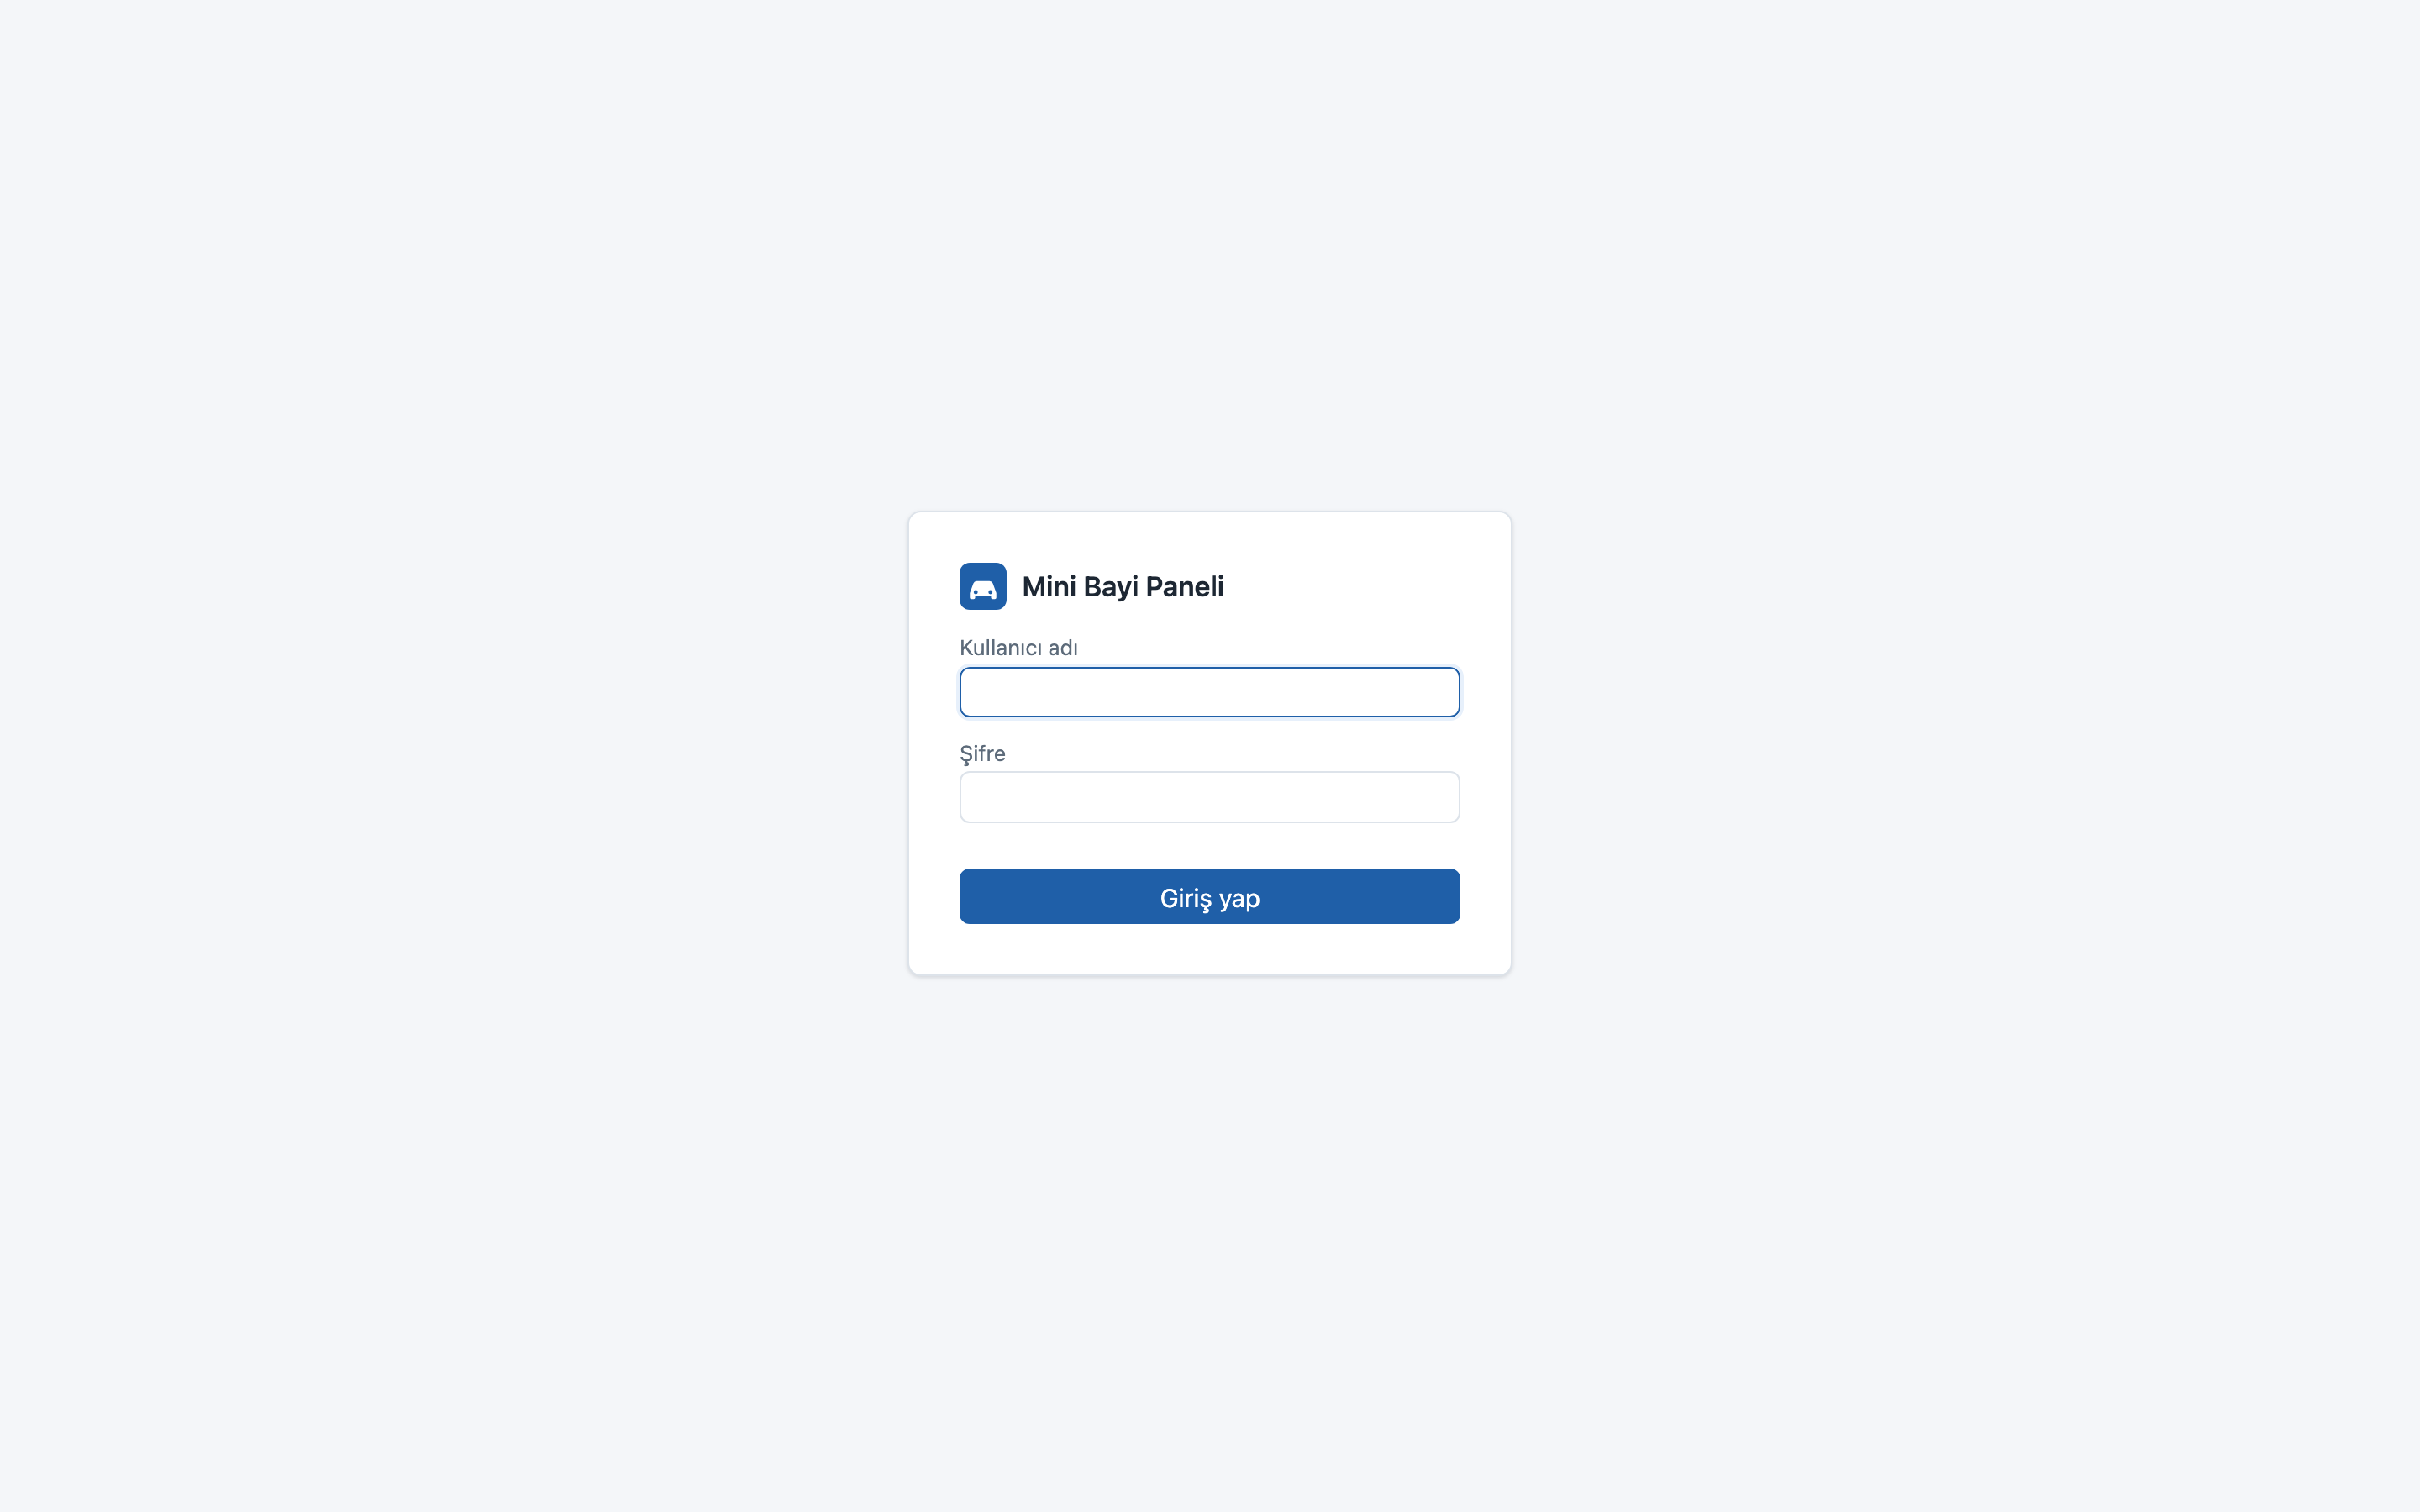
\includegraphics[width=0.75\textwidth]{figures/panel-giris.png}
\caption{Panel giriş ekranı}
\label{fig:giris}
\end{figure}

\begin{figure}[H]
\centering
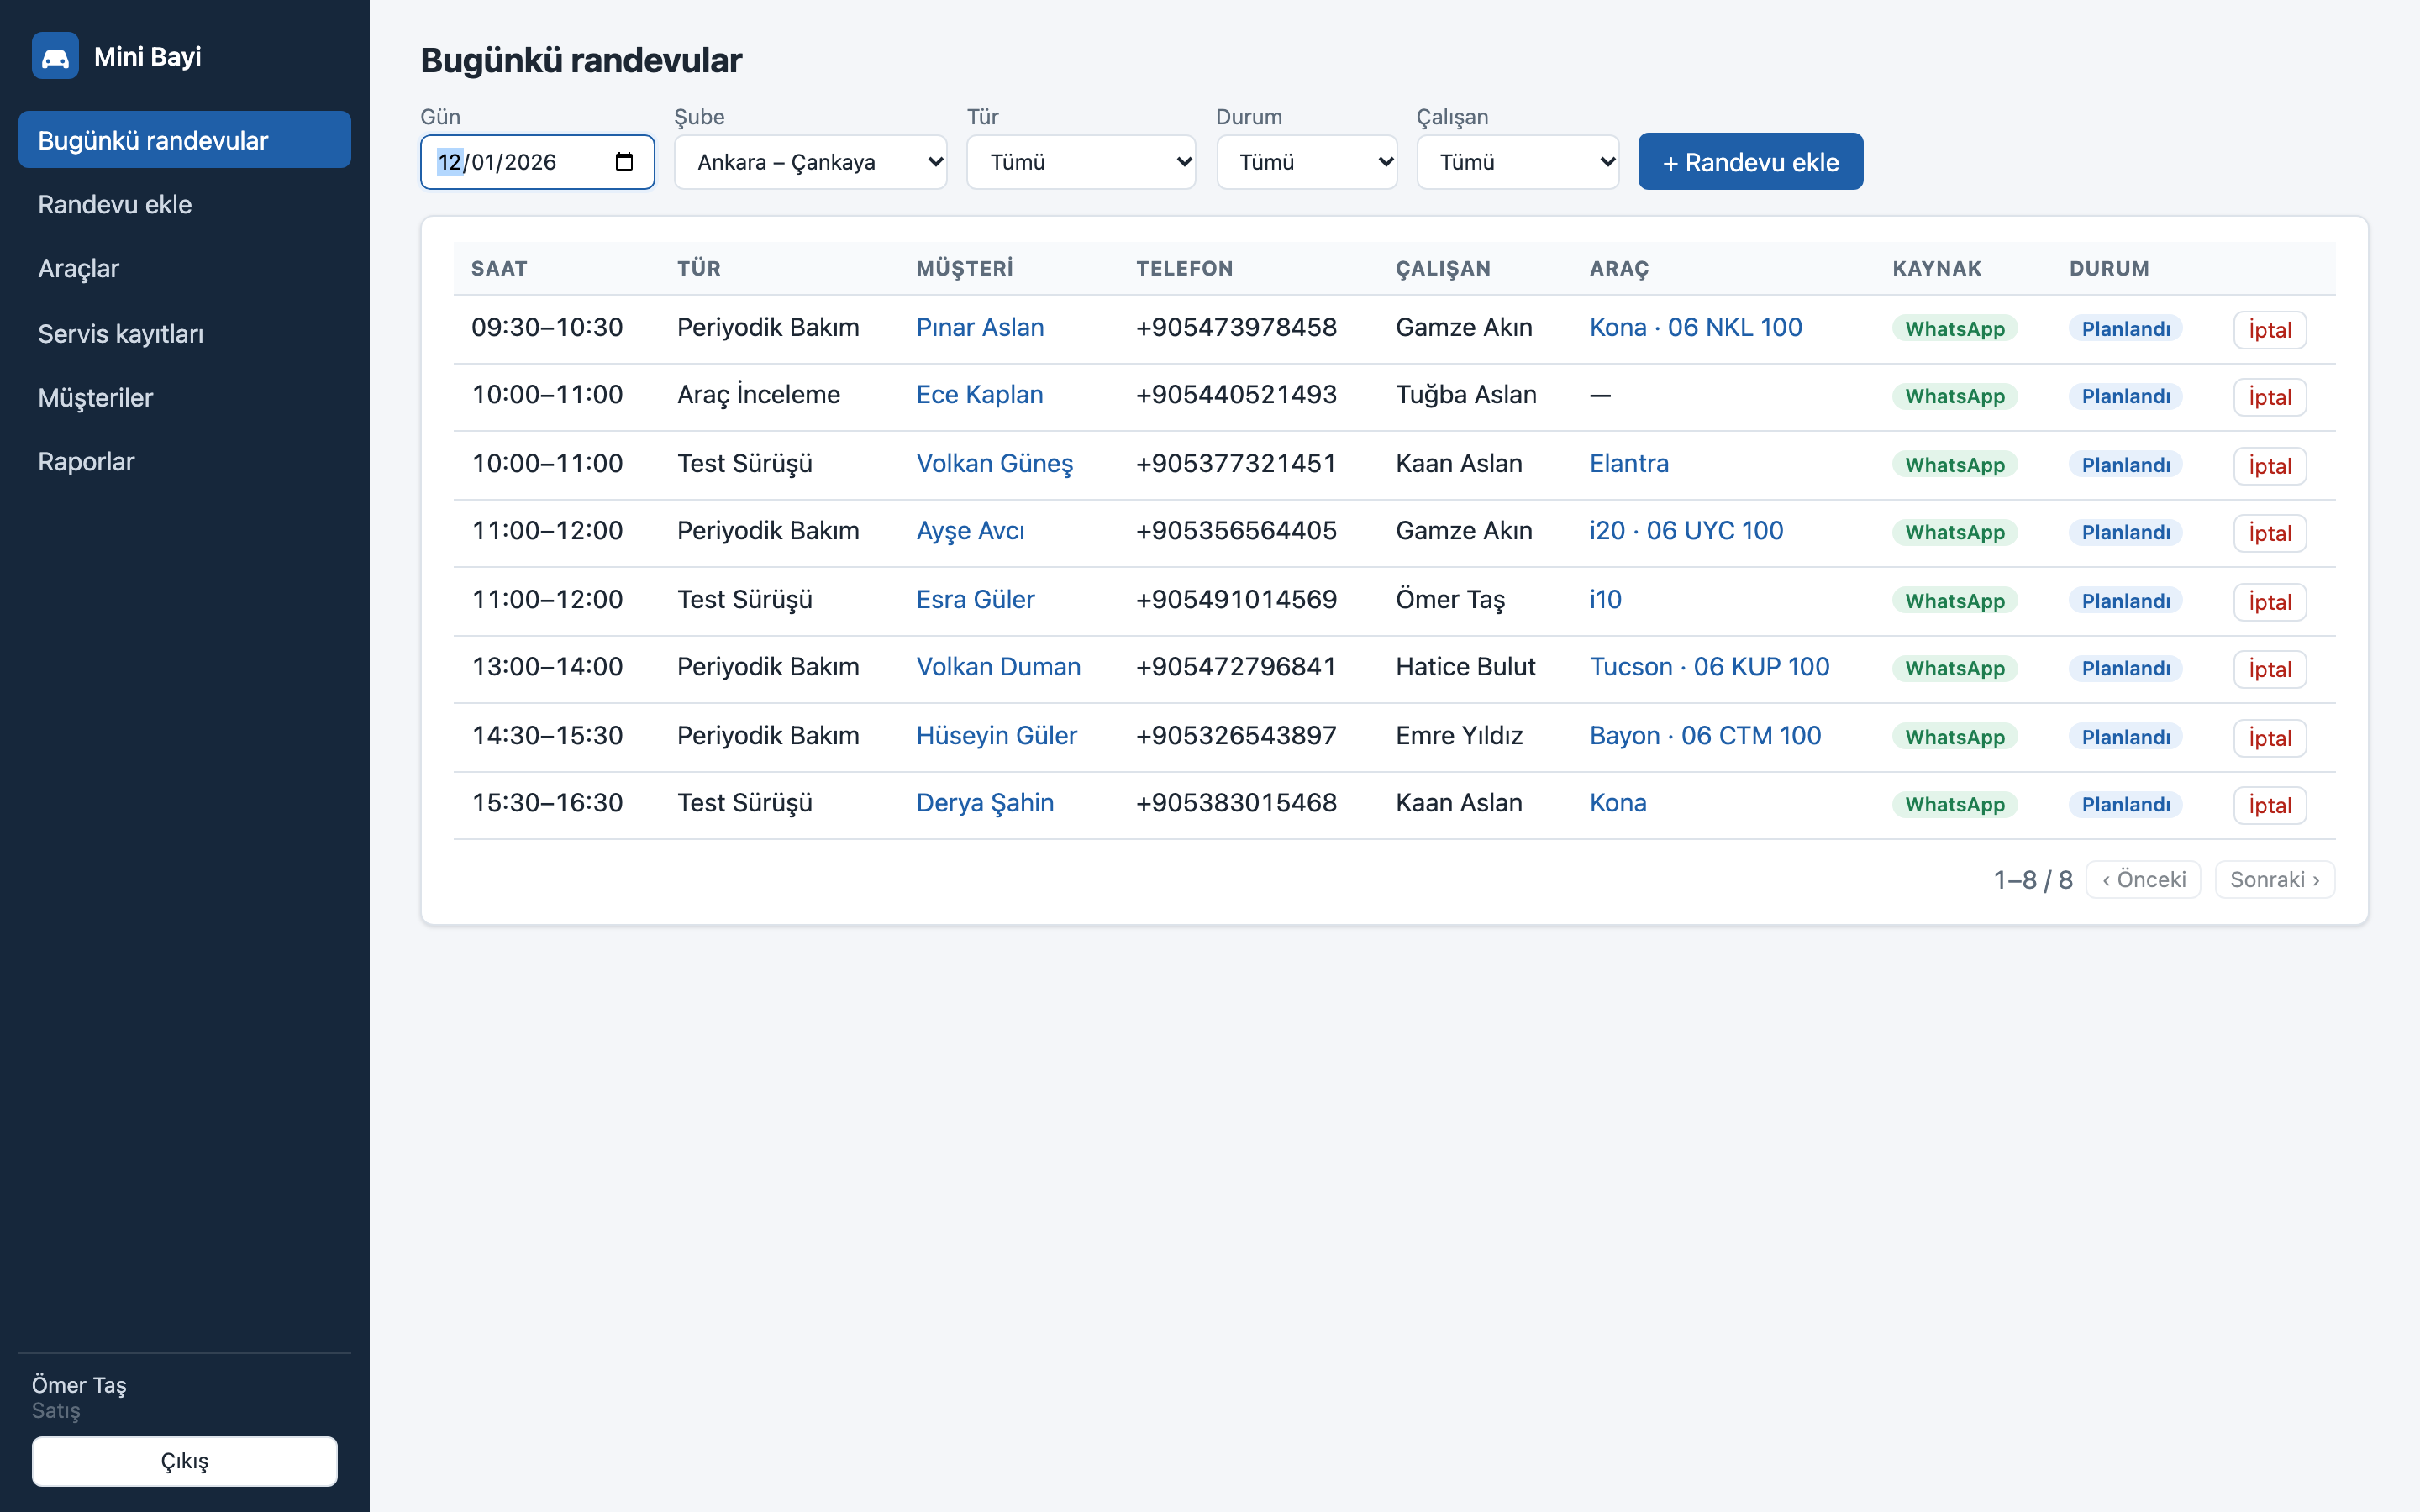
\includegraphics[width=\textwidth]{figures/panel-randevular.png}
\caption{Bugünkü randevular: filtreler ve durum işlemleri}
\label{fig:randevular}
\end{figure}

\begin{figure}[H]
\centering
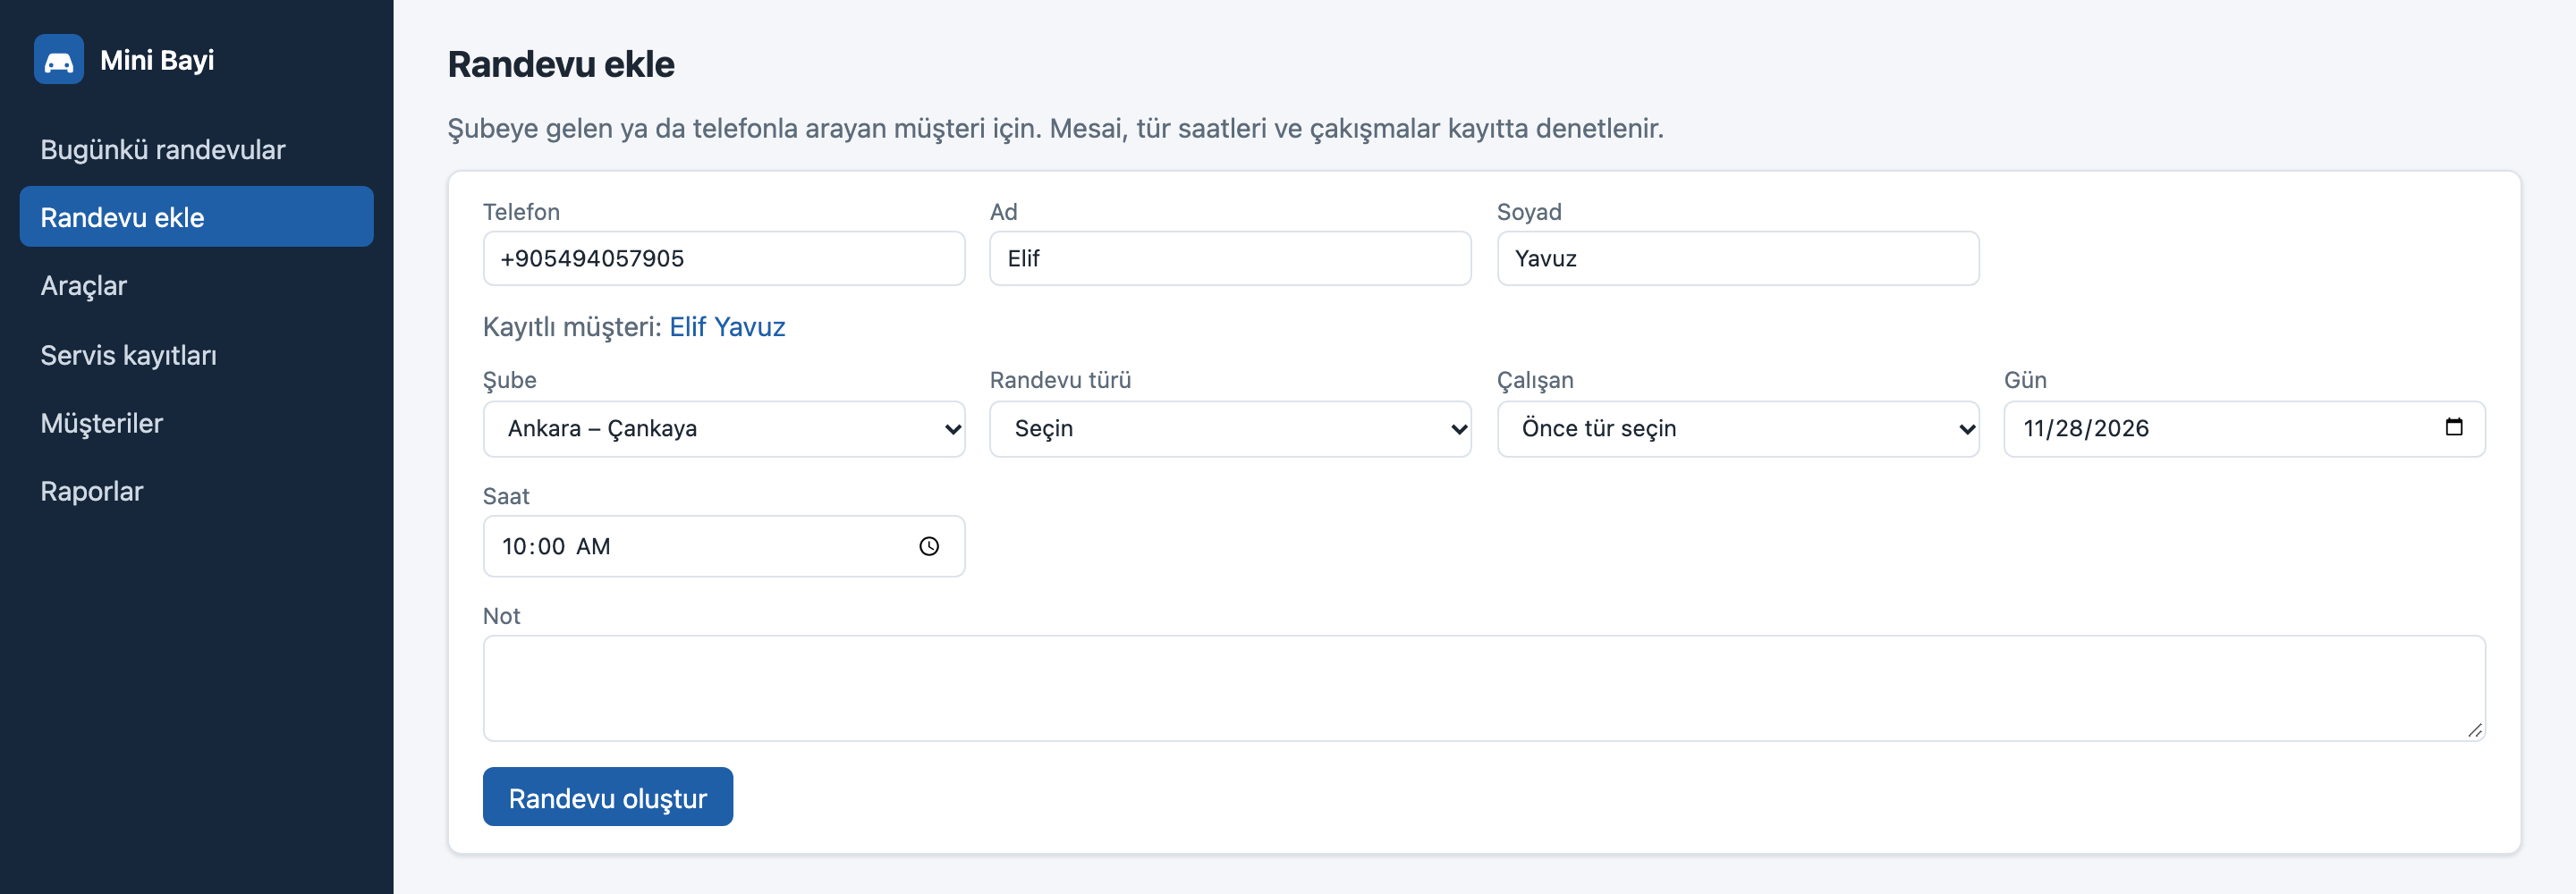
\includegraphics[width=\textwidth]{figures/panel-randevu-ekle.png}
\caption{Müşteri kartından önceden doldurulmuş randevu formu}
\label{fig:randevu-ekle}
\end{figure}

\begin{figure}[H]
\centering
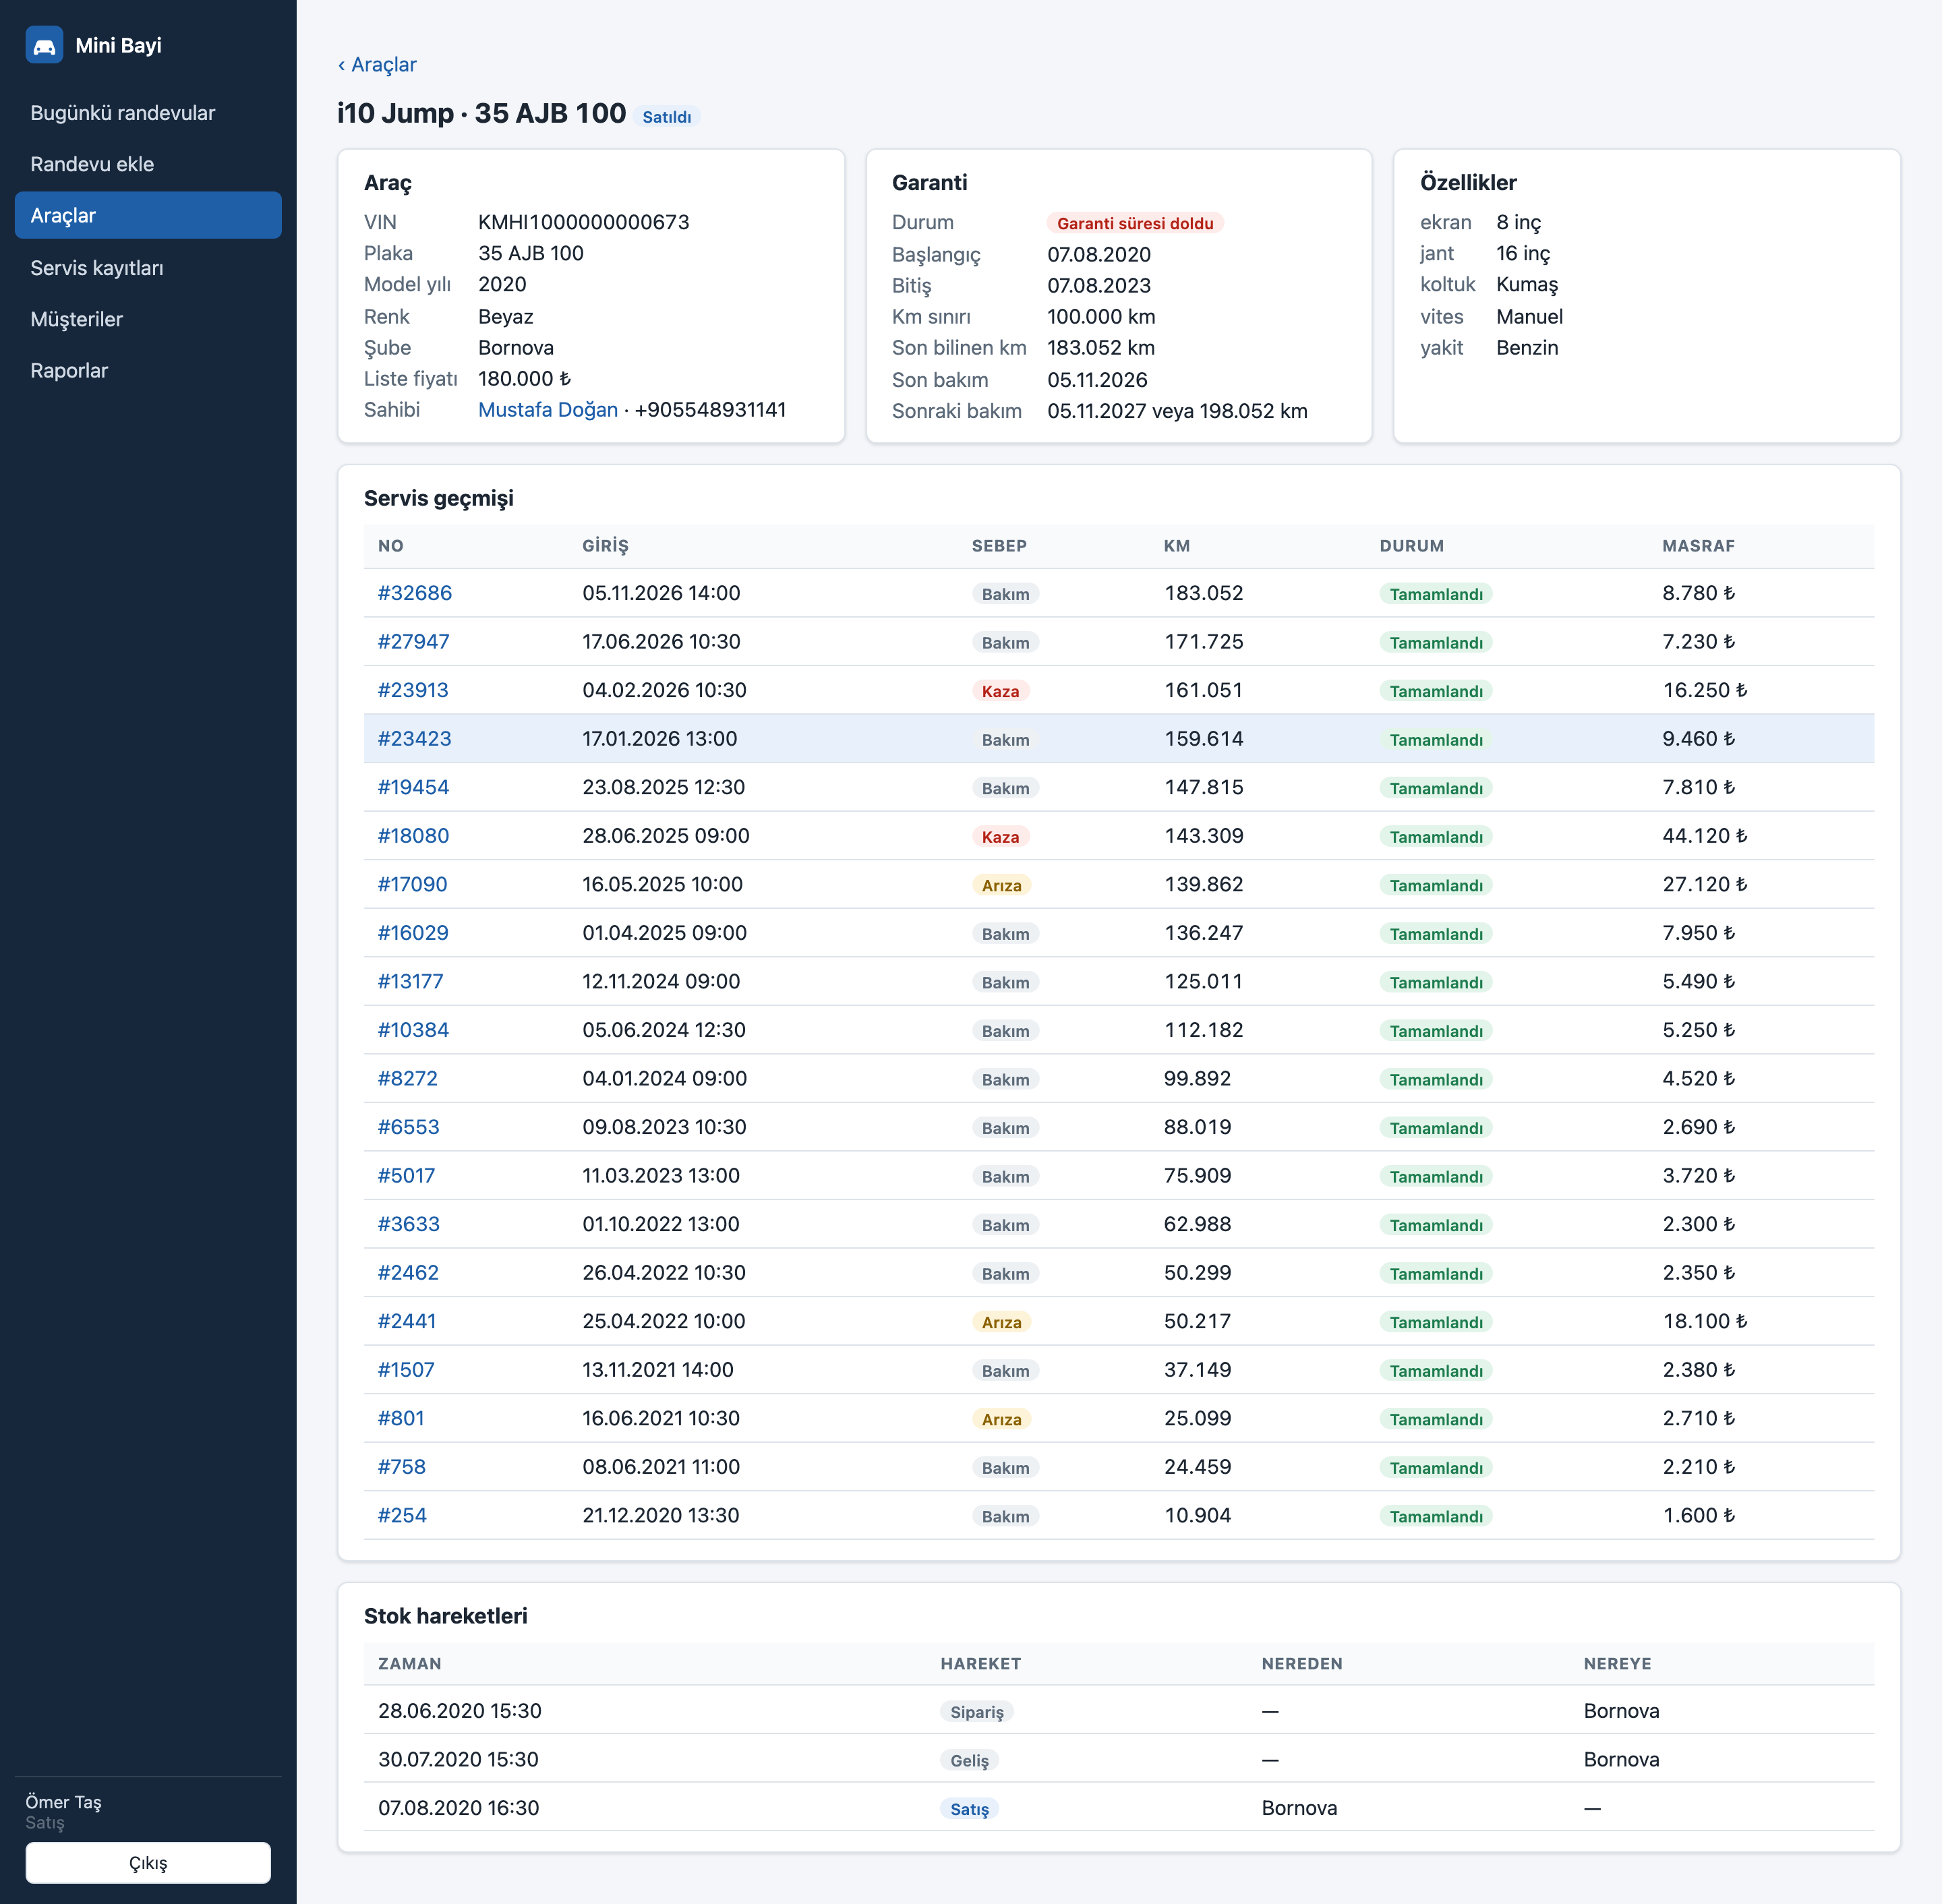
\includegraphics[width=0.95\textwidth]{figures/panel-arac.png}
\caption{Araç detayı: garanti, stok hareketleri ve servis geçmişi}
\label{fig:arac}
\end{figure}

\begin{figure}[H]
\centering
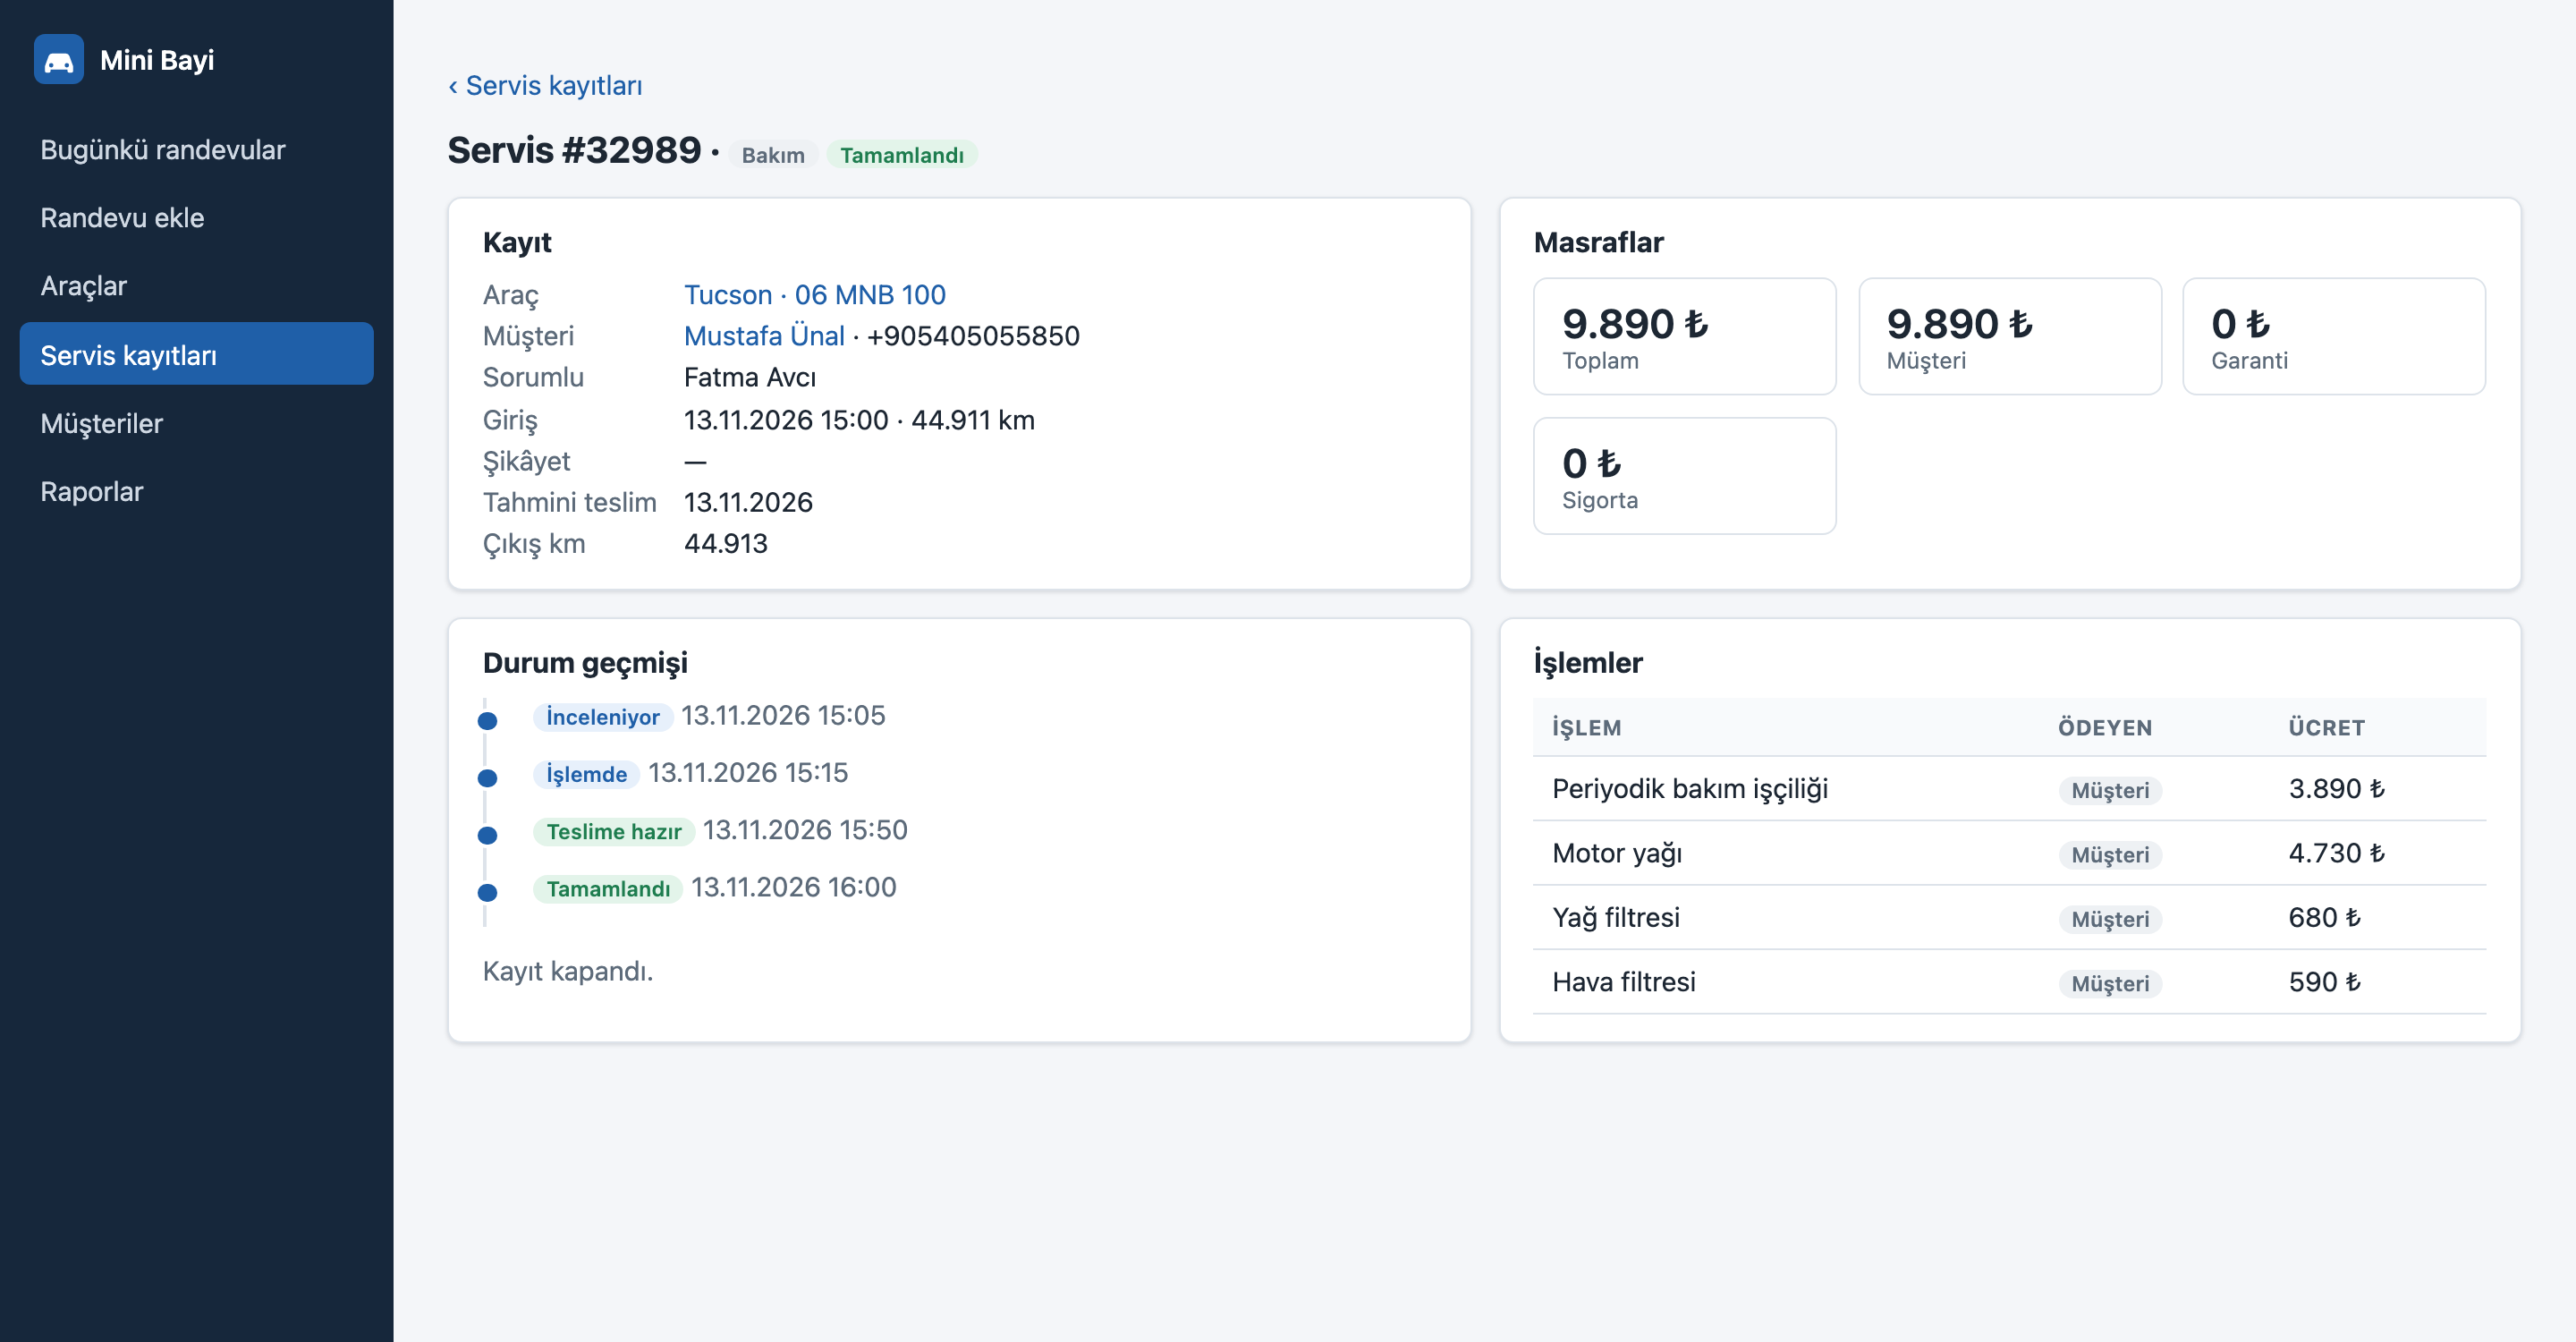
\includegraphics[width=\textwidth]{figures/panel-servis.png}
\caption{Servis kaydı: durum geçmişi ve masraf kırılımı}
\label{fig:servis}
\end{figure}

\begin{figure}[H]
\centering
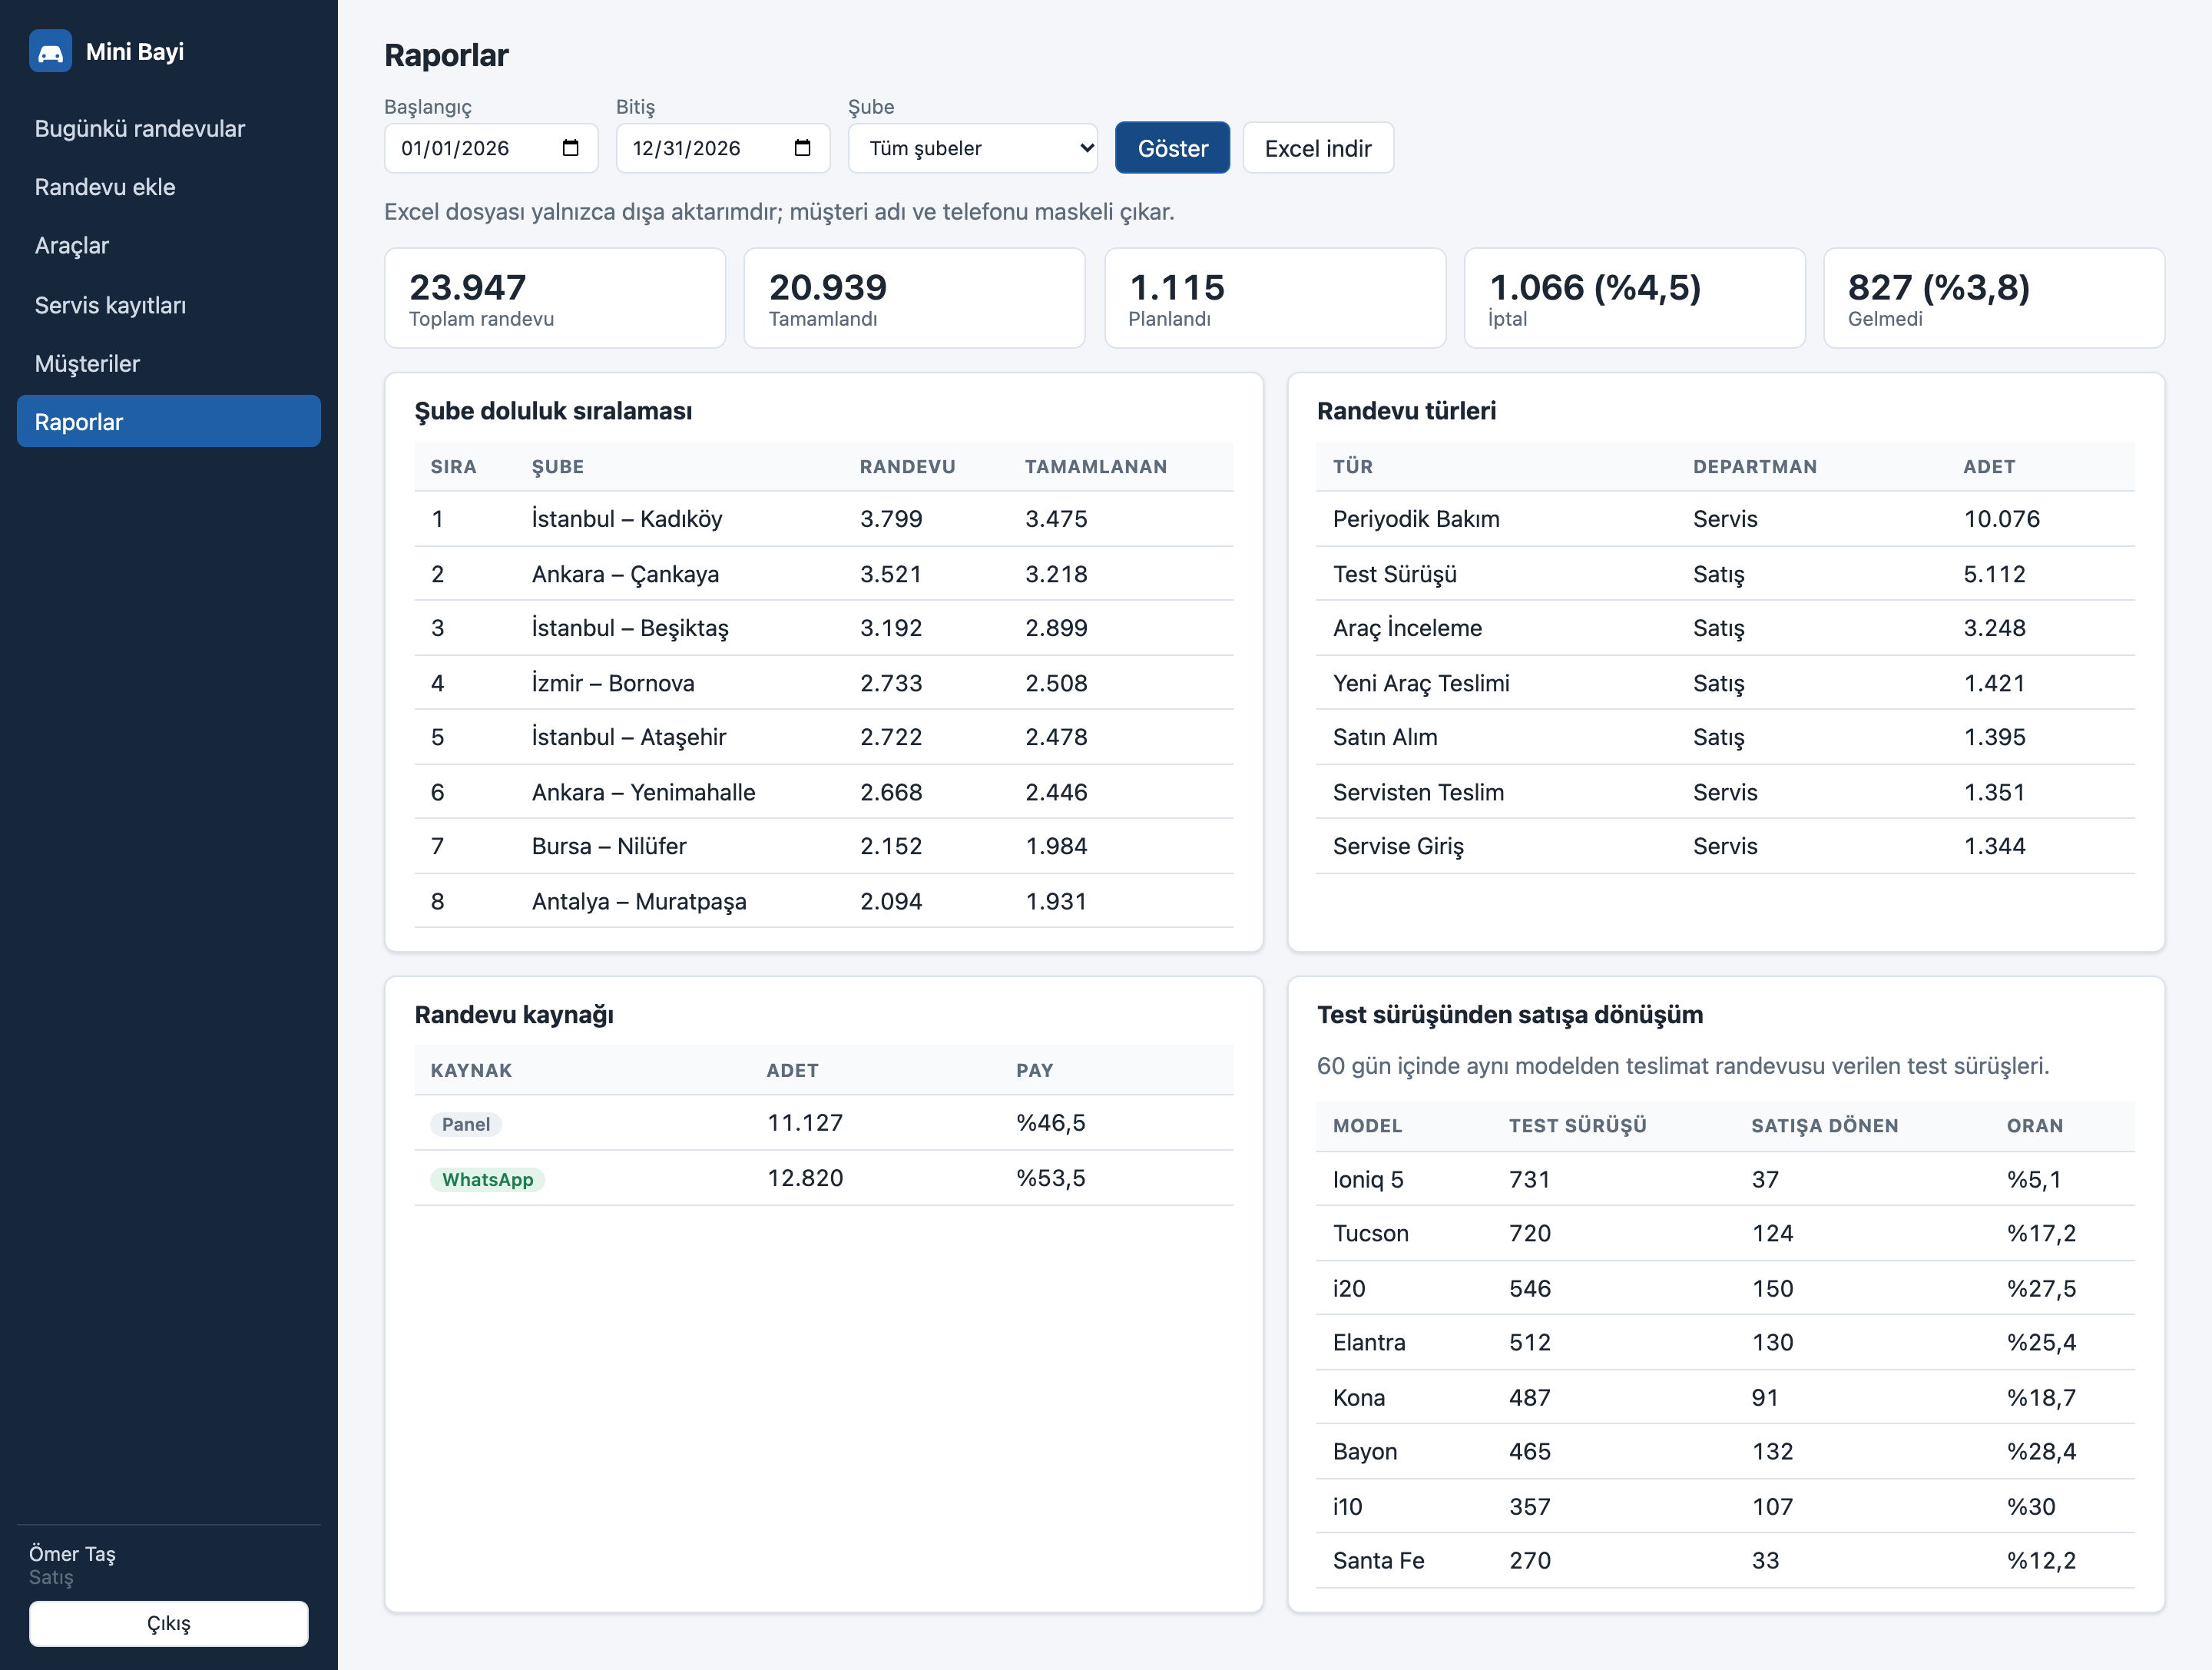
\includegraphics[width=\textwidth]{figures/panel-rapor.png}
\caption{Rapor özeti ve istatistikler}
\label{fig:rapor}
\end{figure}

\begin{figure}[H]
\centering
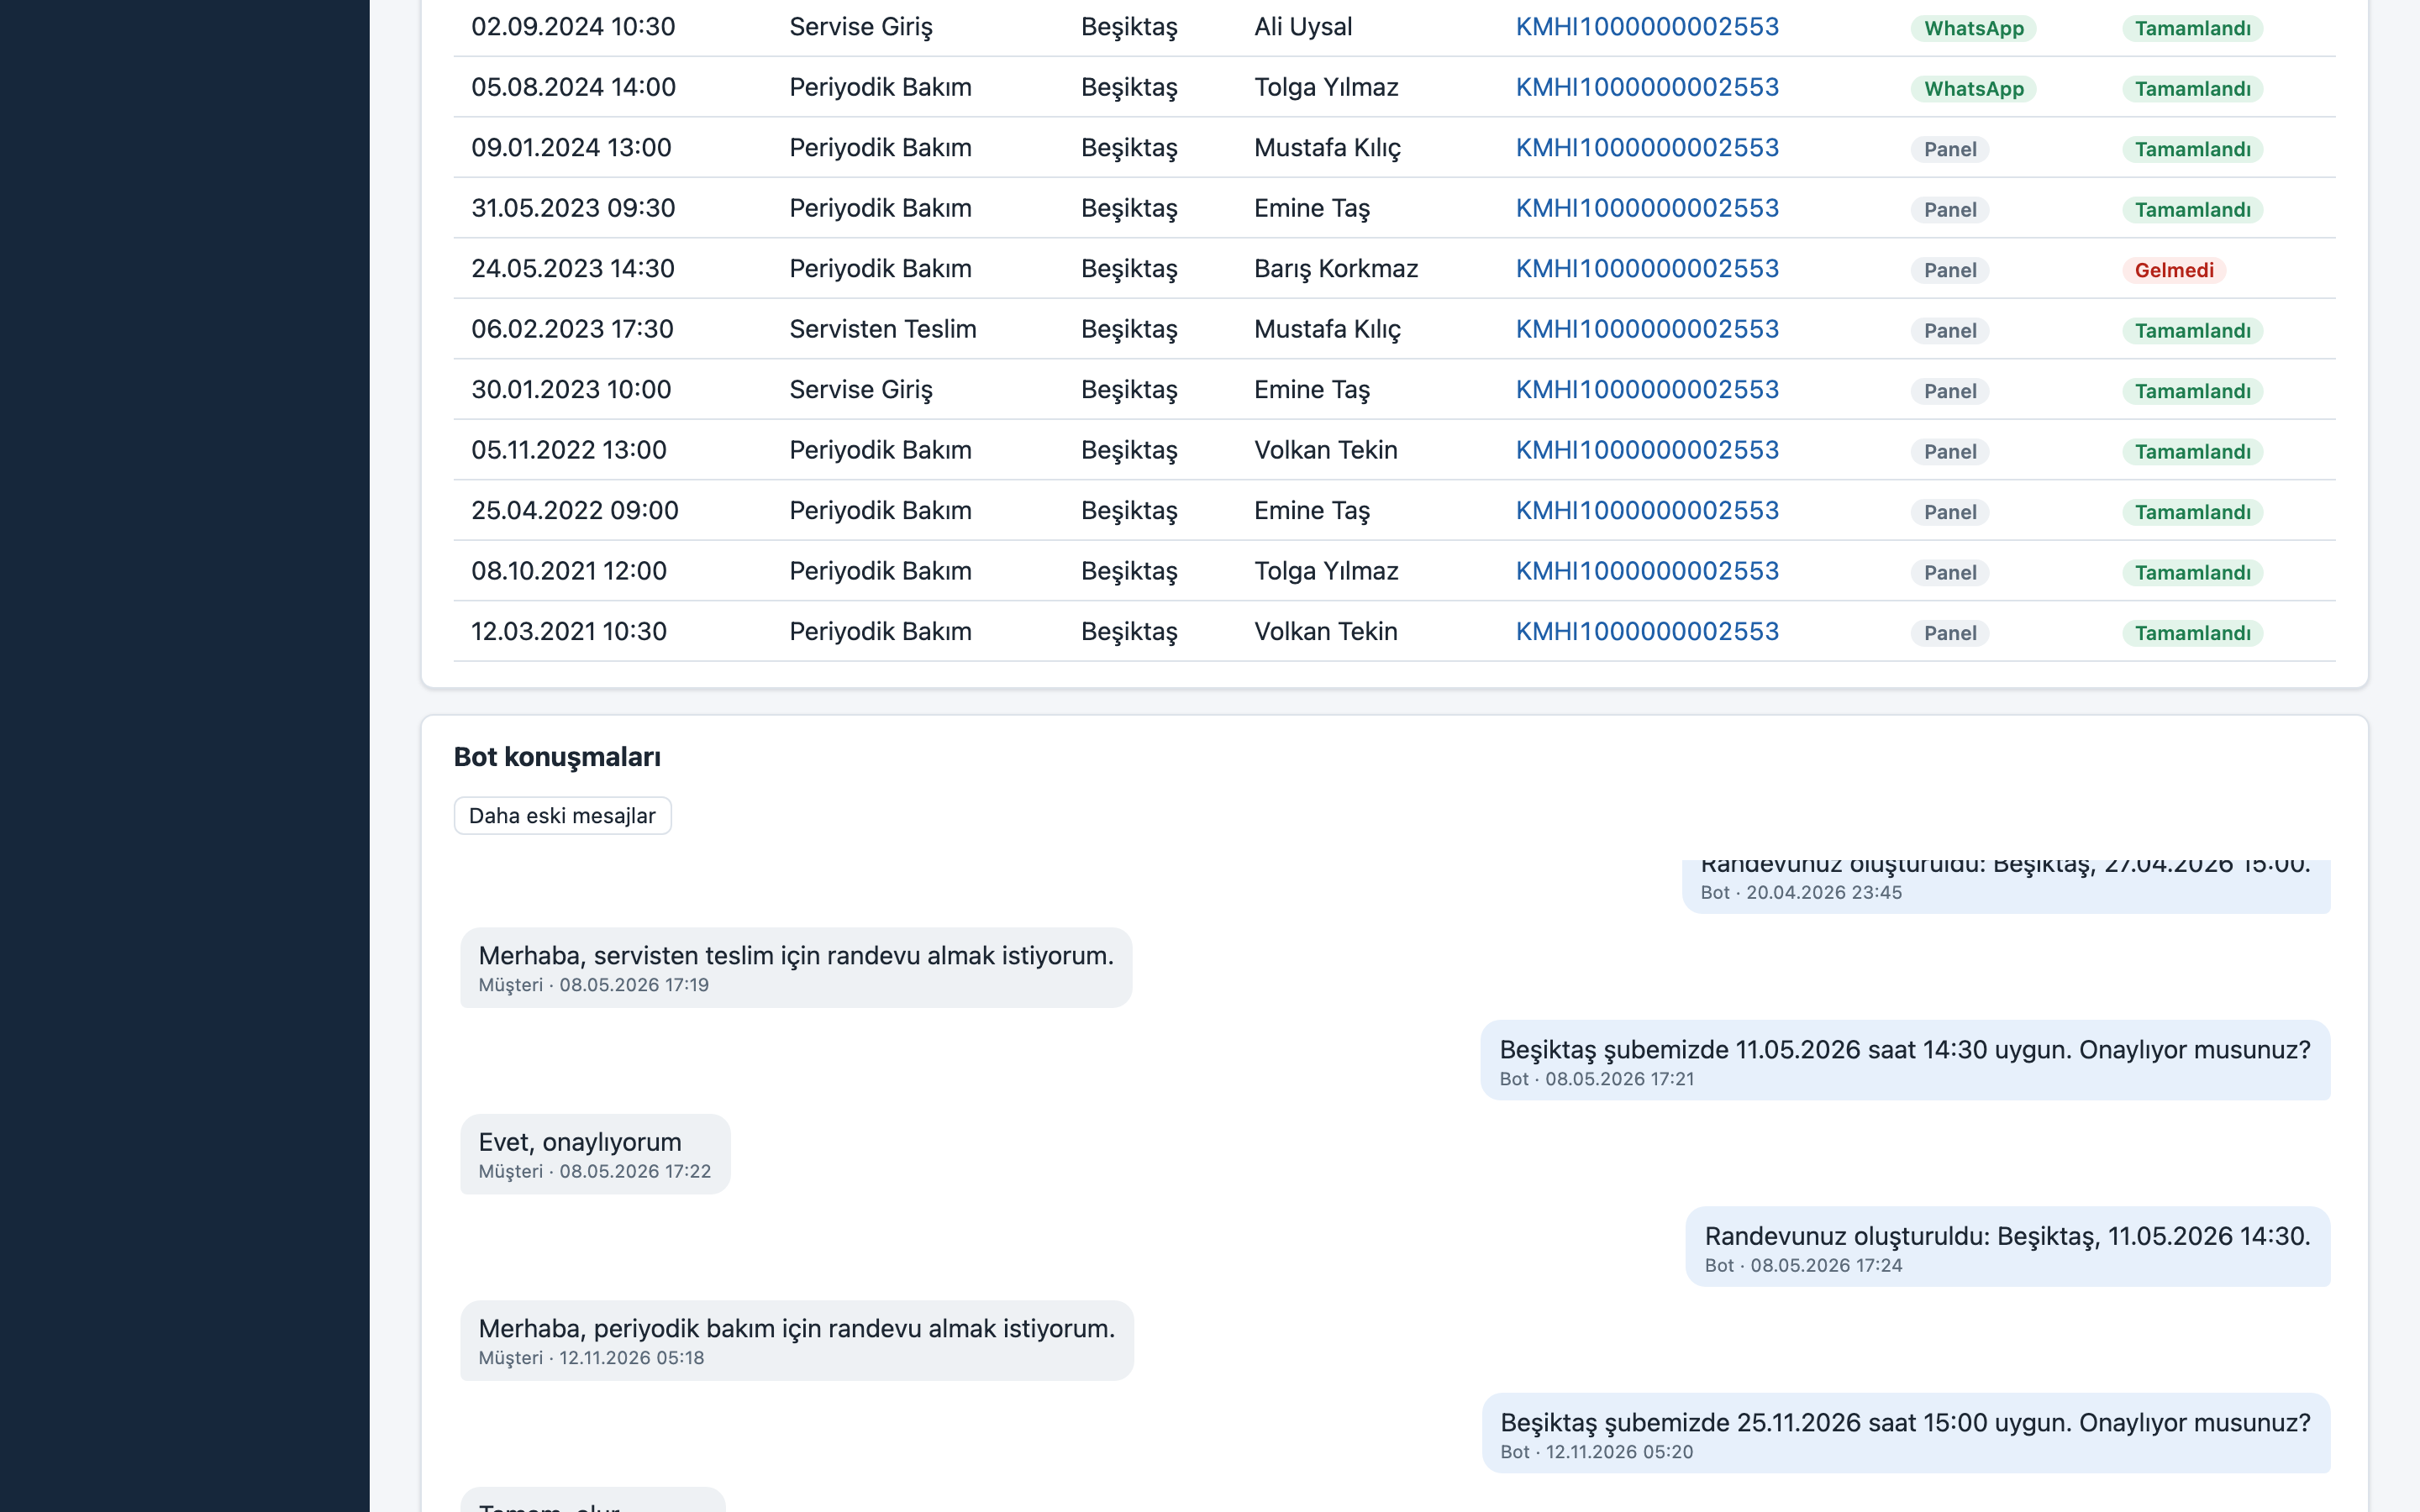
\includegraphics[width=\textwidth]{figures/panel-musteri.png}
\caption{Müşteri kartı ve bot konuşmaları}
\label{fig:musteri}
\end{figure}

\subsection{WhatsApp botu}

\begin{enumerate}[leftmargin=1.4em]
  \item Müşteri: ``Merhaba, Ioniq 5 için test sürüşü randevusu almak istiyorum.''
  \item Bot: Şehir/şube ve gün sorar; \kod{GET /bot/slot} ile boş saatleri listeler.
  \item Müşteri saati seçer; bot \kod{POST /bot/randevu} ile kaydeder.
  \item Onay mesajı: tarih, saat, şube, çalışan.
  \item ``Randevularım'' $\rightarrow$ \kod{GET /bot/randevu}; iptal
        $\rightarrow$ \kod{POST .../iptal}.
  \item Güncelleme: eski randevu \kod{randevu_iptal}, yeni saat
        \kod{musait_slotlar} + \kod{randevu_olustur} ile değiştirilir.
\end{enumerate}

Randevu kuralları modele bırakılmaz: model yalnızca aracı çağırır; DB kuralı
reddederse bot bunu kullanıcıya anlaşılır biçimde söyler.

\begin{figure}[H]
\centering
\IfFileExists{figures/whatsapp.png}{
  \includegraphics[width=0.42\textwidth]{figures/whatsapp.png}
}{
  \fbox{\parbox[c][7cm][c]{0.42\textwidth}{\centering
  WhatsApp ekran görüntüsü\\[2mm]
  \kod{figures/whatsapp.png} dosyasını ekleyin}}
}
\caption{WhatsApp botu ile örnek konuşma (telefon ekran görüntüsü)}
\label{fig:whatsapp}
\end{figure}

\subsection{API sözleşmeleri}

\begin{itemize}[leftmargin=1.2em]
  \item Bot: \kod{docs/api/bot-sozlesmesi.md} --- 8 uç.
  \item Panel: \kod{docs/api/panel-sozlesmesi.md} --- 19 uç.
  \item Ortak zarf: \texttt{\{"ok": true, "veri": ...\}} /
        \texttt{\{"ok": false, "hata": \{ ... \}\}}.
\end{itemize}

\subsection{Çalıştırma}

\begin{lstlisting}[language=bash]
# 1) Sema + sentetik veri (gecici PostgreSQL ile dogrulama)
./scripts/test-db.sh
./scripts/veri-yukle.sh

# 2) Backend
cd backend && ./mvnw package -DskipTests
./scripts/backend-calistir.sh

# 3) Panel demosu (sentetik veri + demo hesaplari)
./scripts/panel-demo.sh

# 4) Kopru
cd kopru && npm install && npm start   # QR ile WhatsApp eslestirme
\end{lstlisting}

\section{Sonuç}

\subsection{Elde edilenler}

\begin{itemize}[leftmargin=1.2em]
  \item 20 tablo, 7 view, 3 trigger ve 13 indeksten oluşan, BCNF'ye
        normalleştirilmiş şema; 660.433 satır sentetik veri.
  \item Bot API (8 uç), panel API (19 uç), WhatsApp köprüsü ve LLM araç döngüsü.
  \item Veritabanında garanti edilen iş kuralları: çakışma, mesai/yetkinlik,
        sahiplik, servis hazırlığı, garanti/ödeme kaynağı, rol/RLS.
  \item 509 otomatik senaryo; üç HTTP paketi, JUnit ve köprü testleri.
  \item Ölçülmüş indeks kazançları: 722$\times$'e varan iyileşme;
        \kod{EXPLAIN (ANALYZE, BUFFERS)} çıktıları tekrarlanabilir.
\end{itemize}

\subsection{Sınırlar ve gelecek işler}

\begin{itemize}[leftmargin=1.2em]
  \item Panelden satış transaction'ı ve servis kaydı açma/teslim uçları kapsam dışı.
  \item Oturumlar bellekte; çok örnekli dağıtımda paylaşılan oturum deposu gerekir.
  \item Docker Compose ile tek komut demo hedefi sonraki adımdır; bu raporda yerel
        betiklerle çalıştırma doğrulanmıştır.
  \item \kod{personel} rolünün bazı tablolarda kolon bazlı yetkisi genişletilebilir
        (şu an tablo bazlı UPDATE).
\end{itemize}

\subsection{Öğrenilenler}

\begin{itemize}[leftmargin=1.2em]
  \item İş kurallarını uygulama koduna değil veritabanına yazmak, yeni bir yazma
        yolu (panel) eklendiğinde bile tutarlılığı korur.
  \item DEFERRABLE constraint trigger, toplu veri yükleme sırası ile katı bütünlük
        arasındaki gerilimi çözer.
  \item \kod{EXCLUDE} + \kod{btree_gist}, çakışma denetimini yarış koşullarından
        bağımsız kılar.
  \item Gerçek HTTP üzerinden test etmek, ``SQL'i elle çalıştırdım''dan çok daha
        güçlü kanıt üretir.
\end{itemize}

\subsection{Ekip iş bölümü}

\begin{table}[H]
\centering
\small
\begin{tabularx}{\textwidth}{@{}l X@{}}
\toprule
Üye & Katkı\\
\midrule
Hüseyin Yiğit USTA & EER/şema/DDL, roller/RLS, indeks analizi, bot API, WhatsApp
köprüsü, LLM, panel API sertleştirmesi, Docker/ortam, test altyapısı\\
Şevda Yağmur ASAL & Panel API ve arayüzü, panel menüleri, Excel raporu, istatistik
sayfası, panel hata düzeltmeleri\\
Ortak & Gereksinim analizi, veri üretici, test senaryoları, rapor\\
\bottomrule
\end{tabularx}
\caption{Ekip iş bölümü}
\label{tab:isbolumu}
\end{table}

% =====================================================================
\begin{thebibliography}{9}
\bibitem{proje} BIL372 Veritabanı Sistemleri, Proje Tanımı ve Ara Rapor,
TOBB ETÜ, 2026.
\bibitem{pg} PostgreSQL 17 Documentation: Constraints, Triggers, Row Security
Policies, \kod{EXPLAIN}. \url{https://www.postgresql.org/docs/17/}
\bibitem{gist} PostgreSQL \kod{btree_gist} extension.
\bibitem{jdk} JDK 17 \kod{com.sun.net.httpserver} documentation.
\bibitem{hikari} HikariCP, Jackson, jBCrypt, fastexcel proje belgeleri.
\bibitem{baileys} Baileys (WhatsApp Web API) 7.0.0-rc13 belgeleri.
\bibitem{llm} Mistral AI ve Google Gemini API belgeleri.
\bibitem{repo} Proje deposu: \url{https://github.com/huseyin-usta/mini-dealership}
\end{thebibliography}

\end{document}
